	\documentclass[a4paper, twoside, 11pt]{article}
\usepackage{amsmath} %matematic package%
\usepackage{textcomp} %for miscellaneous symbols%
%\usepackage{times} %times font%
\usepackage{graphicx} %enhanced support for craphics%
%\usepackage{mathptmx} %use Times as default text font, and provide maths support%
\usepackage{cmap} %mapování znaků - vyhledávání v pdf%
\usepackage[czech]{babel}%CZ%
\usepackage[utf8]{inputenc}%kódování%
\usepackage[T1]{fontenc}%kódování%
\usepackage{multirow}%Multirow table support
\usepackage{float}%Improves the interface for defining floating objects such as figures and tables%
\usepackage{wasysym} %for various glyphs, symbols%

\usepackage{hyperref}
\hypersetup{
    colorlinks=true, %pokud nechci definovat citecolor=black aby byly odkazy citací černé, tak dám colorlinks=false,%
    bookmarks=true,
    linkcolor=black,
    citecolor=black,
    urlcolor=black,
}

%when using LuaLaTex, defining Times Fonts from your system - it has to be named like this%
\usepackage{fontspec}
\selectlanguage{czech}
\setmainfont[Ligatures=TeX,BoldFont={* Bold}] {Times New Roman}
                                
 \setsansfont[Ligatures=TeX,BoldFont={* Bold}]{Times New Roman}
                                      
 \setmonofont{Times New Roman}
 
%\usepackage[italic]{mathastext} %for text in math environment, better looking times then



%for CITATIONS URL to work, it is not needed when you are not using URL label%
\usepackage{url}
\usepackage{csquotes}
\usepackage[style=iso-numeric, backend=bibtex, isbn=true]{biblatex}
\addbibresource{zdroje.bib}
%\DeclareUrlCommand\url{\def\UrlLeft{<}\def\UrlRight{>} \urlstyle{tt}}



\usepackage{biblatex}
%END for citations%

%changing bibliography font%
\renewcommand*{\bibfont}{\fontspec{Times New Roman}}

\usepackage{comment} %For comments%
\usepackage{pdfpages}%for pdf pages%
\usepackage{enumerate}%For lists%
\usepackage{tikz} %For vector graphics%
\usepackage{circuitikz}%For schemes%
\usepackage{pgf} %Post script graphics for tikz%

%pouze funguje v PDFLaTeX%
%\usepackage{tgtermes}%na times font, jiný nefunguje s vyhledáváním a copy%

%

\usepackage{mathrsfs}%packagee for math symbols for Laplace, Z transform etc., usage \mathscr{Z}
\usepackage{upgreek}%for upgreek symbols, specified tau \uptau

%this works only when using PDFLaTeX%
\usepackage[list=true,listformat=simple]{subcaption}
\usepackage[figurename=Obr.,font=small,labelfont=it,textfont=it]{caption} %for renaming figures instead of renewcommand, small for 11pt default is 10pt as needed in word template
\usepackage[tablename=Tab.,font=small,labelfont=it,
            textfont=it]{caption} %for renaming tables instead of renewcommand
            
            %this works with LuaLaTex and fontspec package%
      \DeclareCaptionFont{times}{\fontspec{Times New Roman Italic}}

%labelfont and textfont defined here only works with previous declarecaptionfont times and fontspec%
\captionsetup{labelfont=times, textfont=times, labelsep=space}%no separator in captions
%

%\bibliographystyle{czechiso} %czechiso.bst in folder is needed for this style to work, available at http://www.fit.vutbr.cz/~martinek/latex/czechiso.html%

%\hyperref[label]{text}% Help for targeting labels

\usepackage{chngcntr} %for numbered figures with sections
\usepackage{tocloft}%better TOC

%\usepackage{a4wide}%širší a4%
\usepackage[inner=3cm,outer=2cm,top=2.5cm,bottom=2.5cm,footskip=1cm]{geometry}%for propper margins
\usepackage{textcase}%for making text uppercase without caps \MakeTextUppercase
 
 
\usepackage{titlesec}%for spacing text after sections
\usepackage{parskip}[]%for Workng \parskip

\setlength{\parindent}{0.5cm}%setting indent of paragraph to 0.5cm
\setlength{\parskip}{0em}%setting parskip to 0 for \titleformat to work properly with parskip package
\usepackage{colortbl}%for colored cells
\usepackage{xcolor}%for colors
\definecolor{ctublue}{HTML}{0065BD}%defining ctu color
\definecolor{light_blue}{HTML}{B4C6E7}
\definecolor{light_orange}{HTML}{F8CBAD}
\definecolor{light_green}{HTML}{C6E0B4}
\definecolor{light_red}{HTML}{EA8986}


\titlespacing*{\section}{0em}{1em}{-\parskip}%spacing text after sections from titlesec package
\titlespacing*{\subsection}{0em}{1em}{-\parskip}%spacing text after sections from titlesec package
\titlespacing*{\subsubsection}{0em}{1em}{-\parskip}%spacing text after sections from titlesec package

%when you want sectin/sub/subsub to be black, delete \color{ctublue}
\titleformat{\section}{\color{ctublue}\fontspec{Times New Roman}\fontsize{15}{15}\bfseries}{\thesection}{2.1em}{}%defining title sizes by word template
\titleformat{\subsection}{\color{ctublue}\fontspec{Times New Roman}\fontsize{14}{14}\bfseries}{\thesubsection}{1.53em}{}%defining title sizes by word template
\titleformat{\subsubsection}{\color{ctublue}\fontspec{Times New Roman}\fontsize{13}{13}\bfseries}{\thesubsubsection}{1em}{}%defining title sizes by word template

\usepackage{ctable}%imports xtable with booktabs
\usepackage{multicol}


%%change in previous commands 2.1 em , 1.53em and 1em to 1em to be easy indented not the same
\begin{document}
\fontspec{Times New Roman}

\counterwithin{figure}{section}%changing counter of figure, at each section the numbering resets
\counterwithin{table}{section}%changing counter of table, at each section the numbering resets
\counterwithin{equation}{section}%changing counter of equation, at each section the numbering resets
\renewcommand{\thefigure}{\thesection~-~\arabic{figure}}%defining style of countering
\renewcommand{\thetable}{\thesection~-~\arabic{table}}
\renewcommand{\theequation}{\thesection~-~\arabic{equation}}

\renewcommand*{\cftsecdotsep}{1}  % use dots in the section entries and their step
\renewcommand*{\cftsubsecdotsep}{1}
\renewcommand*{\cftsubsubsecdotsep}{1}
\renewcommand*{\cftsecnumwidth}{4em} % increase space for Roman numerals
\renewcommand*{\cftsubsecnumwidth}{4em} %numbering width
\renewcommand*{\cftsubsubsecnumwidth}{4em} %numbering width
\renewcommand*{\cftsubsubsecindent}{0em}%no indent for subsubsection
\renewcommand*{\cftsubsecindent}{0em}%no indent for subsection
\renewcommand*{\cftsecindent}{0em}%no indent for subsection

\renewcommand*{\cftfigdotsep}{1}  % use dots in the figure entries and their step
\renewcommand*{\cftfignumwidth}{4em}
\renewcommand*{\cftfigindent}{0em}

\renewcommand*{\cfttabdotsep}{1}  % use dots in the figure entries and their step
\renewcommand*{\cfttabnumwidth}{4em}
\renewcommand*{\cfttabindent}{0em}

\renewcommand{\cftsecfont}{\fontspec{Times New Roman}\large \bfseries}
\renewcommand{\cftsubsecfont}{\fontspec{Times New Roman}}
\renewcommand{\cftsubsubsecfont}{\fontspec{Times New Roman}}

\renewcommand{\cftfigfont}{\fontspec{Times New Roman}}
\renewcommand{\cfttabfont}{\fontspec{Times New Roman}}

\renewcommand*\contentsname{\textcolor{ctublue}{\MakeTextUppercase{\fontspec{Times New Roman}Obsah}}}
\renewcommand{\listtablename}{{\fontspec{Times New Roman}\textcolor{ctublue}{\MakeTextUppercase{{Seznam tabulek}}}}}
\renewcommand{\listfigurename}{{\fontspec{Times New Roman}\textcolor{ctublue}{\MakeTextUppercase{{Seznam obrázků}}}}}



%\renewcommand{\thefigure}{\arabic{section}.\arabic{figure}}%changing figure name to be section.subsection. but do no reset
\setcounter{figure}{0}

\begin{titlepage}
	\begin{center}

\begin{figure}[H]
	\begin{center}
		
\includegraphics[scale=1]{files/symbol_cvut_konturova_verze.pdf}
	\end{center}
\end{figure}
	{\Large{\textbf{ČESKÉ VYSOKÉ UČENÍ TECHNICKÉ V~PRAZE}}}\\
	{\textbf{Fakulta elektrotechnická}}\\
	
	\vspace{3cm}
	
	
	{\Large\textbf{Osvětlení podzemních garáží}}\\
	\vspace{0.3cm}
	{\large\textbf{OC Trnávka, Vlašim}}
	\vspace{1cm}
	
	Projektová dokumentace\\
	\vspace{0.4cm}
	
	\end{center}
	
	\vspace{3cm}
	
	%\noindent Studijní program: Elektrotechnika, Energetika a Management\\
	%\noindent Studijní obor: Aplikovaná elektrotechnika
	\noindent Investor: PEG spol. s~r.o., IČO: 45278784\\
	\noindent Zpracovatelé: Jan Hnát\\
	\hspace*{2.2cm}Petr Zakopal, IČO: 08990107
	\vspace{0.5cm}
	
	
	\vfill
	
\begin{center}

	\large{\textbf{Jan Hnát}}\\
	\large{\textbf{Petr Zakopal}}\\
	\large{\textbf{Praha 2021}}
	\end{center}
\end{titlepage}


\newpage
%\pagenumbering{arabic} to arabic page numbering
\pagenumbering{gobble} %disabling page numbering

\pagenumbering{Roman}
\setcounter{page}{2}%%3 NUTNO řešit dle zadání etc.

\newpage
\tableofcontents
\flushbottom %vyčištění stránky
\newpage
\vspace{0pt}
\listoffigures %seznam obrázků
\listoftables
\flushbottom
\newpage

\pagenumbering{arabic} %to arabic page numbering - enabling page numbering after gobble which disabled page numbering
\setcounter{page}{1}

\section{Úvod}
	Projektová dokumentace, prezentace a přílohy jsou volně dostupné v~průběhu  letního semestru 2021 na webové adrese \url{https://ptzk.cz/tpr} a slouží pouze ke studijním účelům. Jakékoliv kopírování a šíření díla bez předchozího souhlasu autorů je zakázáno. Výjimku tvoří citace.
	
	\section{Zadání projektu}
	\textbf{Klient:}\\
		Objednávám rekonstrukci/výměnu osvětlení podzemních garáží v~OC Trnávka, Vlašim. Osvětlení je ve špatném technickém stavu – viz periodická rev. zpráva. Kabeláž je také nevyhovující. Osvětlení také již nevyhovují novým hygienickým normám pro osvětlení garážových stání.\\ \\
		
		\noindent \textbf{Projektové zadání:}\\
		\noindent Zrealizujte výměnu osvětlení ve výše uvedené lokalitě, včetně vypracování technického projektu.\\ 
		\noindent Požaduji dodávku „ na klíč“, včetně vyřízení všech legislativních formalit.\\ 
\noindent Práce musí probíhat za provozu garáží s~minimálním omezením provozu (max. uzavření některých ploch).\\ 
\noindent Dodávka bude obsahovat mj. i dodávku všeho materiálu, demontáž starého osvětlení a zajištění ekologické likvidace starého materiálu. O~provedení ekologické likvidace požadujeme předat likvidační protokol.\ 
\noindent Ukončení projektu požaduji do 30.10.2021\\ 
\noindent Požaduji vyřízení dotace z~obecních zdrojů – fond na revitalizaci veřejně prospěšných objektů.\\ 
\noindent Součástí předání bude výchozí revizní zpráva elektro a protokol o~dodržení hygienických limitů.\\ 
\noindent Platba za projekt bude 100\% po předání projektu a ukončení zkušebního provozu, se splatností faktury 120 dnů.\\ \\

			\noindent \textbf{Podrobnosti k~projektu:}
				\begin{enumerate}
					\item připojení na síť 3x400/230V TN-S, přípojný bod je vzdálen 150 m, vede průleznými kabelovými kanály,
					\item otevírací doba garáží je 8.00-22.00, v~nočních hodinách jsou garáže zavřené, mohou však probíhat práce,
					\item průjezdová výška garáží je 2,5 m,
					\item výška stropu pro osvětlení je 3,5m,
					\item cesty pro pěší a chodby nesmí být zastavěny, uzavřeny, nebo nijak jinak omezeny,
					\item v~garážích není signál GPS.
				\end{enumerate}
\section{Strategie - business}
	\subsection{Deklarace záměru}
		\subsubsection{Mise}
		Výměna stávajícího nevyhovujícího osvětlení v~podzemních garážích OC Trnávka za nové vyhovující. Součástí výměny svítidel je taktéž výměna stávajícího nevyhovujícího kabelového rozvodu elektrické energie napájející rekonstruované osvětlení.
		\subsubsection{Vize}
		Při rekonstrukci osvětlení dojde ke správné výměně svítidel, která již nevyhovují odpovídajícím normám a příslušným právním předpisům. Díky modernizaci kabelových rozvodů napájících osvětlení dojde k~minimalizaci vzniku možného požáru či výpadku osvětlení.\par
		Projekt rekonstrukce bude ukončen, předán a uveden do provozu do 30.10.2021. Výměna osvětlení a kabeláže bude provedena tak, že nebude nutné osvětlení, kromě drobných servisních oprav, alespoň 9 let rekonstruovat.
		
	\subsection{stav „AS IS“}
		Vnitřní osvětlení garáží OC Trnávka se nachází v~nevyhovujícím stavu. Nejsou splněny aktuálně platné hygienické normy a příslušné právní předpisy. Kabeláž je ve stavu nevhodném pro dlouhodobý provoz. K~dispozici je pouze nevyhovující a neúplná dokumentace o~stávajícím stavu elektroinstalace.
	\subsection{stav „TO BE“}
		Osvětlení včetně odpovídající elektroinstalace v~podzemních garážích OC Trnávka se nyní nachází ve stavu vyhovujícím aktuálně platným normám a příslušným právním předpisům. \par
		Z~důvodu modernizace došlo taktéž k~výměně stávajících rozvaděčů za modernizované řešení s~podporou online monitoringu a možnosti automatické regulace osvětlení.\par
		Došlo ke zvýšení zrakového komfortu při pobytu v~garážích. Modernizované řešení zvyšuje hodnotu garážového stání a může být nabídnuto dlouhodobé parkování zákazníků za zvýšenou cenu.\par
		Je vypracována podrobná odpovídající dokumentace. Je dodán, instalován a zprovozněn software na online podporu a monitoring. SW na monitoring je vybaven podrobnou dokumentací pro možné rozšíření systému.
	\subsection{SMART}
		\subsubsection{Specific}
			Byl přesně popsán problém, který je nutné řešit - výměna stávajícího osvětlení v~podzemních garážích OC Trnávka a výměna nevyhovující kabeláže. Toto řešení bylo doplněno o~výměnu rozváděčů a další minoritní prvky, které  vylepšují řešení hlavního problému.
		\subsubsection{Measurable}
			Řešení je měřitelné pomocí OOU a metrik posaných v~sekci \ref{sec:plan_metrik}. Tento projekt lze také změřit počtem aktuálně vyměněných svítidel, které jsou napojena na rekonstruovanou kabeláž a rekonstruované rozváděče.
		\subsubsection{Aligned}
			Zákazník považoval hlavně rekonstrukci a zajištění legislativy a dokumentace, čehož bylo dosaženo.
		\subsubsection{Realistic}
			Řešení je realistické a prakticky v~80 \% bezúdržbové. Díky předchozí analýze bylo zjištěno, že nedochází k~rapidní degradaci použitých materiálů. Další celková rekonstrukce je plánována v~roce 2051.
		\subsubsection{Timed}
			Časový rámec je stanoven v~harmonogramu dle \ref{sec:gantt}. Předložený harmonogram vykazuje nízkou míru flexibility.
	\subsection{Obchodní přínos}
		\subsubsection{Náklady}
			Finance vyčleněné na tento projekt je nutné rozdělit na nákup materiálu a služeb, na legislativní úkony a na odměny pro zaměstnance. Náklady jsou částečně kryty z~fondu pro revitalizaci veřejně prospěšných objektů.
			
			\begin{table}[H]
				\begin{tabular}{ !{\vrule width 2pt} c | c | c | c  !{\vrule width 2pt}}\noalign{\hrule height 2pt}
				položka & počet (ks, m) & cena 1 ks & cena (Kč)\\ \noalign{\hrule height 2pt}
				projektant elektro &\multicolumn{2}{c|}{}& 32000\\ \hline
				projektant elektro kontrola &\multicolumn{2}{c|}{}& 12000\\ \hline
				automatizační technik &\multicolumn{2}{c|}{}& 23000\\ \hline
				software developer & \multicolumn{2}{c|}{}& 20000\\ \hline
				team 1 - řídící pracovník na pracovišti & \multicolumn{2}{c|}{}& 46000\\ \hline
				team 1 - pracovník 1 & \multicolumn{2}{c|}{}& 42000\\ \hline
				team 1 - pracovník 2 & \multicolumn{2}{c|}{}& 42000\\ \hline
				team 1 - pracovník 3 & \multicolumn{2}{c|}{}& 42000\\ \hline
				team 1 - pracovník 4 & \multicolumn{2}{c|}{}& 42000\\ \hline
				team 1 - pracovník 5 & \multicolumn{2}{c|}{}& 42000\\ \hline
				team 1 - pracovník 16 & \multicolumn{2}{c|}{}& 42000\\ \hline
				
				team 2 - řídící pracovník na pracovišti &\multicolumn{2}{c|}{}& 46000\\ \hline
				team 2 - pracovník 1 &\multicolumn{2}{c|}{}& 42000\\ \hline
				team 2 - pracovník 2 &\multicolumn{2}{c|}{}& 42000\\ \hline
				team 2 - pracovník 3 &\multicolumn{2}{c|}{}& 42000\\ \hline
				team 2 - pracovník 4 &\multicolumn{2}{c|}{}& 42000\\ \hline
				team 2 - pracovník 5 &\multicolumn{2}{c|}{}& 42000\\ \hline
				team 2 - pracovník 16 &\multicolumn{2}{c|}{}& 42000\\ \hline
				
				team 3 - pracovník 1 &\multicolumn{2}{c|}{}& 28000\\ \hline
				team 3 - pracovník 2 &\multicolumn{2}{c|}{}& 28000\\ \hline
				kontaktní osoba GTWD &\multicolumn{2}{c|}{}& 7000\\ \hline
				právní zařizovatel &\multicolumn{2}{c|}{}& 12000\\ \hline
				objednavatel materiálu a prací &\multicolumn{2}{c|}{}& 4000\\ \hline
				revizní technik &\multicolumn{2}{c|}{}& 7000\\ \hline
				zpracovatel dokumentace &\multicolumn{2}{c|}{}& 4000\\ \hline
				účetní projektu &\multicolumn{2}{c|}{}& 4000\\ \hline
				vedoucí projektu &\multicolumn{2}{c|}{}& 32000\\ \hline
				EUROPA-LED-5100-236-4K & 300 & 1165 & 349500\\ \hline
				CYKY-J 3x2,5 RE PRAKAB & 5000 & 35 & 175000\\ \hline
				CYKY-J 3x1,5 RE PRAKAB & 1000 & 25 & 25000\\ \hline
				CYKY-J 5x2,5 RE PRAKAB & 3000 & 55 & 165000\\ \hline
				CYKY-J 5x6 RE PRAKAB & 1500 & 85 & 127500\\ \hline
				ostatní montážní materiál &\multicolumn{2}{c|}{}& 35000\\ \hline
				vybavení rozváděčů &\multicolumn{2}{c|}{}& 28000\\ \hline
				pronájem plošiny &\multicolumn{2}{c|}{}& 20000\\ \hline
				ekologická likvidace a pronájem kontejneru 1 &\multicolumn{2}{c|}{}& 15000\\ \hline
				SW &\multicolumn{2}{c|}{}& 15000\\ \hline
				ostatní náklady &\multicolumn{2}{c|}{}& 21000\\ \noalign{\hrule height 2pt}
				celková cena &\multicolumn{2}{c|}{}& 1568000\\ \hline
				rozpočet &\multicolumn{2}{c|}{}& 1588000\\ \hline
				
				\end{tabular}
			\caption{Rozpočet verze s~LED svítidly}
			\end{table}
			
						\begin{table}[H]
				\begin{tabular}{ !{\vrule width 2pt} c | c | c | c  !{\vrule width 2pt}}\noalign{\hrule height 2pt}
				položka & počet (ks, m) & cena 1 ks & cena (Kč)\\ \noalign{\hrule height 2pt}
				projektant elektro &\multicolumn{2}{c|}{}& 32000\\ \hline
				projektant elektro kontrola &\multicolumn{2}{c|}{}& 12000\\ \hline
				automatizační technik &\multicolumn{2}{c|}{}& 23000\\ \hline
				software developer & \multicolumn{2}{c|}{}& 20000\\ \hline
				team 1 - řídící pracovník na pracovišti & \multicolumn{2}{c|}{}& 46000\\ \hline
				team 1 - pracovník 1 & \multicolumn{2}{c|}{}& 42000\\ \hline
				team 1 - pracovník 2 & \multicolumn{2}{c|}{}& 42000\\ \hline
				team 1 - pracovník 3 & \multicolumn{2}{c|}{}& 42000\\ \hline
				team 1 - pracovník 4 & \multicolumn{2}{c|}{}& 42000\\ \hline
				team 1 - pracovník 5 & \multicolumn{2}{c|}{}& 42000\\ \hline
				team 1 - pracovník 16 & \multicolumn{2}{c|}{}& 42000\\ \hline
				
				team 2 - řídící pracovník na pracovišti &\multicolumn{2}{c|}{}& 46000\\ \hline
				team 2 - pracovník 1 &\multicolumn{2}{c|}{}& 42000\\ \hline
				team 2 - pracovník 2 &\multicolumn{2}{c|}{}& 42000\\ \hline
				team 2 - pracovník 3 &\multicolumn{2}{c|}{}& 42000\\ \hline
				team 2 - pracovník 4 &\multicolumn{2}{c|}{}& 42000\\ \hline
				team 2 - pracovník 5 &\multicolumn{2}{c|}{}& 42000\\ \hline
				team 2 - pracovník 16 &\multicolumn{2}{c|}{}& 42000\\ \hline
				
				team 3 - pracovník 1 &\multicolumn{2}{c|}{}& 28000\\ \hline
				team 3 - pracovník 2 &\multicolumn{2}{c|}{}& 28000\\ \hline
				kontaktní osoba GTWD &\multicolumn{2}{c|}{}& 7000\\ \hline
				právní zařizovatel &\multicolumn{2}{c|}{}& 12000\\ \hline
				objednavatel materiálu a prací &\multicolumn{2}{c|}{}& 4000\\ \hline
				revizní technik &\multicolumn{2}{c|}{}& 7000\\ \hline
				zpracovatel dokumentace &\multicolumn{2}{c|}{}& 4000\\ \hline
				účetní projektu &\multicolumn{2}{c|}{}& 4000\\ \hline
				vedoucí projektu &\multicolumn{2}{c|}{}& 32000\\ \hline
				EUROPA-PC-280-EP, 2x80W & 300 & 1504 & 451200\\ \hline
				Osram LUMILUX L 13W/840 T5 G5 neutrální bílá 4000K 517mm & 600 & 100 & 60000\\ \hline
				CYKY-J 3x2,5 RE PRAKAB & 5000 & 35 & 175000\\ \hline
				CYKY-J 3x1,5 RE PRAKAB & 1000 & 25 & 25000\\ \hline
				CYKY-J 5x2,5 RE PRAKAB & 3000 & 55 & 165000\\ \hline
				CYKY-J 5x6 RE PRAKAB & 1500 & 85 & 127500\\ \hline
				ostatní montážní materiál &\multicolumn{2}{c|}{}& 35000\\ \hline
				vybavení rozváděčů &\multicolumn{2}{c|}{}& 28000\\ \hline
				pronájem plošiny &\multicolumn{2}{c|}{}& 20000\\ \hline
				ekologická likvidace a pronájem kontejneru 1 &\multicolumn{2}{c|}{}& 15000\\ \hline
				SW &\multicolumn{2}{c|}{}& 15000\\ \hline
				ostatní náklady &\multicolumn{2}{c|}{}& 21000\\ \noalign{\hrule height 2pt}
				celková cena &\multicolumn{2}{c|}{}& 1729700\\ \hline
				rozpočet &\multicolumn{2}{c|}{}& 175000\\ \hline
				
				\end{tabular}
			\caption{Rozpočet verze s~zářivkovými svítidly}
			\end{table}
		
		\subsubsection{Přínosy}
			%Modernizované osvětlení a kabeláž bude vyhovovat normám a příslušným právním předpisů. Dojde ke zlepšení zrakového komfortu při pobytu v garážích. Nebude nutnost rekonstruovat osvětlení a kabeláž v garážích v tomto rozsahu po dobu minimálně 12 let.
			Dojde k~získání dalších zkušeností s~prací uvnitř veřejně prospěšného objektu, kde není možné uzavřít celý areál. Akce rekonstrukce přínáší možnost objevu dalších nevyhovujících instalací v~OC Trnávka a navázání delší spolupráce v~rámci servisu a rekonstrukce.\par
			Se zákazníkem je možné převážně navázat spolupráci v~rámci servisu osvětlení. V~ceně projektu je zahrnuta celková preventivní revize instalace po jednom roce v~provozu. Při této revizi je doporučená kontrola stavu rozváděčů. Smlouva taktéž obsahuje on-line a telefonní podporu. \par
			Součástí smlouvy není kontrola po polovině předpokládané doby provozu ani celková kontrola po 80 \% předpokládané doby životnosti svítidel a zdrojů světla.
	%	\subsubsection{Zhodnocení}
			%Garáže budou působit příjemněji na zákazníky, dojde ke zvýšení hodnoty garáží. Tato přidaná hodnota v budoucnu může umožnit pronajímat trvalá parkovací místa za vyšší cenu. Očekává se nárůst poptávky po této službě.
			
		%\subsubsection{Benefit}
			%Dojde ke zvýšení spokojenosti zákazníků při návštěvě OC Trnávka. Vylepšená osvětlenost může nalákat podnitele, uvažující o provozování podnikatelské činnosti v podzemních garážích, např. mytí aut, autokosmetika, detailing apod.
	\subsection{SWOT}	
	
	\begin{table}[H]
	\catcode`\-=12%aby fungovalo c-line v kategorii -= 12
		\resizebox{1 \textwidth}{!}
		{
		\begin{tabular}{  !{\vrule width 2pt} c !{\vrule width 2pt} m{2cm} !{\vrule width 2pt} m{2cm} | m{2cm} | m{2cm} | p{2cm}  !{\vrule width 2pt} p{2cm} | m{2cm} | m{2cm} | m{2cm} !{\vrule width 2pt} p{2cm} !{\vrule width 2pt} m{2cm}  !{\vrule width 2pt} m{2cm} !{\vrule width 2pt} }\noalign{\hrule height 2pt}
	\multicolumn{2}{!{\vrule width 2pt}c !{\vrule width 2pt}}{SWOT} & \multicolumn{4}{c !{\vrule width 2pt}}{Silné stránky} & \multicolumn{4}{c !{\vrule width 2pt}}{Slabé stránky} & Součet\\ 	\noalign{\hrule height 2pt}
 \multicolumn{2}{!{\vrule width 2pt}c !{\vrule width 2pt}}{}  & tradice & široké portfolio & schopný marketing & propracovaná interní komunikace &vyšší věkový průměr zaměstnanců & cena služeb & méně schopné účetní oddělení & závislost na zahraničních měnách  & \cellcolor{gray} \\ \noalign{\hrule height 2pt}
 \multirow{15}{*}{Příležitosti} & okolní technické průmyslové školy & 4 & 3 & 5 & 0 & 0 & 0 & -3 & 0 & 9 \\ \cline{2-11}
  &zamezení vstupu/složitejší vstup konkurence na trh & 5 & 4 & 2 & 0 & 0 & -3 & -5 & -3 & -4  \\ \cline{2-11}
  & kancelářští pracovníci mohou pracovat odkudkoliv & 0 & 5 & 3 & 5 & -2 & 0 & -3 & 0 & 8 \\ \cline{2-2}
  & růst trhu automatizace & 5 & 5 & 4 & 3 & -3 & -1 & -3 & -5 & 3  \\ \noalign{\hrule height 2pt}
  
 \multirow{15}{*}{Hrozby} & nemoc pracovníků & 0 & 4 & 0 & 3 & -5 & 0 & -3 & 0 & -1    \\ \cline{2-11}
   & neplatící zákazníci & 5 & 5 & 3 & 2 & 0 & -5 & -5 & -4 &  1  \\ \cline{2-11}
  & odebrání licencí/povolení & 1 & 4 & 0 & 3 & 0 & -3 & -3 & -3 & -1   \\ \cline{2-11}
  & zvýšení cen produktů od dodavatelů & 3 & 3 & 1 & 0 & -2 & 3 & -5 & -5 &   \\ \noalign{\hrule height 2pt}
  \multicolumn{2}{!{\vrule width 2pt}c !{\vrule width 2pt}}{Součet} & 22 & 33 & 17 & 15 & -15 & -11 & -28 & -21 &  \cellcolor{gray}  \\ 	\noalign{\hrule height 2pt}
	
		\end{tabular}
		}
		\caption{Kvantitativní SWOT}\label{tab:swot}
		\end{table}
		

		%rozepsání SWOT%
		\subsubsection{Silné stránky}
		Naše firma je na trhu již 20 let a za tu dobu si vybudovala tradici a získala četné reference v~oboru, je to naše velmi silná stránka. Protože se nespecializujeme na jednu část a své porfolio diverzifikujeme, je možné se uplatnit jak ve stavbě rodinných domů, tak v~průmyslových nebo VPO. Jsme zastánci kvalitního marketingu a proto se neustále zdokonalujeme v~rámci marketingu a snažíme se ho udržet na vysoké úrovni. Díky vývoji nástroje GTWD jsme vytvořili interní komunikační infrastrukturu, která nám umožňuje komunikovat efektivněji, než konkurenční firmy.	
		
		\subsubsection{Slabé stránky}
			Máme zkušené pracovníky, ale tato zkušenost je vykoupena vyšším věkem, který zvedá průměr. Ovšem v~posledních letech se trend začíná postupně měnit a průměrný věk snižovat. Protože nabízíme velmi komplexní služby s~řadou podpůrných balíčků, máme vyšší cenu než konkurence. Naše účetní oddělení je méně schopné, kvůli tomu mohou vznikat problémy. Tohoto problému jsme si vědomni a snažíme se ho řešit doplňujícími školeními. Protože přibližně 60 \% našich zákazníků jsou zahraniční firmy, jsme značně závislí na kurzech USD a EUR.
		
		
		\subsubsection{Příležitosti}
		V~okrese naší firmy se nachází řada kvalitních průmyslových škol, jejichž absolventy pravidelně zaměstnáváme na letních brigádách a v~případě jejich zájmu s~nimi v~budoucnu uzavíráme HPP. Díky nutnosti certifikátů, povolení a oprávnění (např. ITI) je vstup na některá z~našich částí portfolioa konkurenci ztížený. Výhoda používaných moderních technologií umožňuje práci kancelářských nebo dokonce i z~části projekčních pracovníků odkudkoliv. Trh automatizační techniky a globální potřeba automatizace dává příležitost expanze naší firmy.
		
		\subsubsection{Threats}
			Může dojít k~onemocnění některých našich klíčových zaměstnacnů a to může způsobit nepříznivé změny harmonogramu. Problém se také vyskytuje u~neplatících zákazníků, nebo zákazníků požadující příliš dlouhé doby splatnosti faktur. Pokud by došlo k~četným problémům ve firmě, může dojít k~odebrání potřebných licencí a certifikátů nutných k~vykonávání klíčových služeb. Pokud dojde ke zvýšení cen produktů našich dodavatelů, jsme nuceni zvýšit taktéž cenu projektu. Značné množství projektů realizujeme dodavatelským způsobem. Většinou nejsme přímými výrobci používaných elektrotechnických zařízení.
			
			\subsubsection{Vyhodnocení SWOT}
				Jak je možné pozorovat na tab. \ref{tab:swot}, původní příležitost „zamezení vstupu/složitější vstup konkurence na trh“ je spíše hrozbou než příležitostí. Podobné špatné určení hrozby je u~„neplatící zákazníci“, ovšem tato hodnota je relativně nevypovídající, protože je velmi blízko rozhodovacímu bodu. Bude považováno, že je stále hrozba.
		
		
		\begin{comment}
		\subsubsection{Strengths}
			Projekt je vypracováván českými odborníky, jež mají zkušenosti v~oboru. Materiál na realizaci projektu je využíván pouze kvalitní, od ověřených dodavatelů. Projekt je převážně realizován, protože stávající osvětlení garáží a kabeláž jsou v~nevyhovujícím stavu z~pohledu norem a právních předpisů. Pokud by nedošlo k~rekonstrukci, jsou tyto normy dále porušovány a to není správné. Je tedy nizká míra rizika zrušení projektu. Je také nízká šance zrušení projektu v~polovině realizace, došlo by k~znefunkčnění celého podzemního komplexu osvětlení a byla by nutná masivní odstávka. 90 \% pracovníků podílející se na tomto projektu je z~jedné firmy, tudíž není nutná další komunikace s~cizími firmami, tudíž se uspoří čas, který by byl jinak potřebný k~obchodním jednáním. Firma HnaZak má zkušenosti s~realizací komplexních projektů zahrnující dodávky na klíč.
		\subsubsection{Weaknesses}
			Prakticky na celou realizaci projektu je nutné vyžadovat pracovníky s~dostatečnou kvalifikací. Montéři musí disponovat s~dostatečnou kvalifikací dle vyhlášky 50/1978 Sb. Za doby pandemie je nutné testovat pracovníky firmy na COVID-19. Je nutná investice do testů. Je problém se sháněním těchto testů, nedisponujeme kontakty na objednávku testů. Firma HnaZak nemá kapacitu zařízení, aby bylo možné vozit materiál každý den na pracoviště a omezení odkládacích a pracovních ploch na pracovišti, protože není povoleno uzavřít garáže, nás omezuje. Nutnost více pracovníků montérů. Aby byl dodržen harmonogramm je nutné zavést noční směny. Tudíž zvýšit plat pracovníků ochotných pracovat v~noci. Je třeba pracovat také při otevřeném OC, je tedy omezený prostor na odkládání materiálu v~podzemních garážích OC Trnávka, protože garáže není možné uzavřít kompletně. Firma HnaZak nedisponuje vysokozdvižnými plošinami typu, který je třeba u~montáže osvětlení do předem dané výšky. Je omezena výška vjezdu do garáží. 
		\subsubsection{Opportunities}
		V~okolí není firma sdružující komplexní služby, které zákazník požaduje, je velmi vysoká šance na zakoupení služeb u~naší firmy s~komplexním balíčkem. Osvětlení vnitřních prostor v~OC Trnávka je také zastaralé, pokud budou s~naší prací a systémem klienti spokojeni, je možnost získat nabídku na další zakázku od OC Trnávka. Pracovnící firmy HnaZak získají zkušenosti s~prací ve veřejně prospěšném objektu, kde nesmí dojít k~omezení pohybu osob. Návrh a výpočet projekce elektroinstalace a osvětlení je proveden dle platných norem a právních předpisů, které se velmi často nemění, je tedy zajištěna dlouhodobá stálost správného návrhu. Možnost snížení spotřeby energie zákazníka při použití dlouhodobě ekonomicky výhodných svítidel. Příležitost získat pro klienta vysokou hodnotu příspěvku z~fondu pro revitalizaci veřejně prospěšných budov. Zákazník si může tudíž dovolit nákladnější návrh a zvýší se hodnota zakázky a finanční zisk z~této zakázky. Je vysoká míra spolehlivosti získání dotace z~fondu pro revitalizaci veřejně prospěšných objektů.
		\subsubsection{Threats}
		Je nutný vícesměnný provoz, je potřeba více kvalifikovaných pracovníků, tím je větší šance, že se zaměstnanci nakazí COVID-19. Nedostatečné množsvtí potřebného navrhnutého materiálu na skladě dodavatele. Dojde ke zpoždění potřebné minimální dodávky materiálu. Pronajímatel vysokozdvižné plošiny má k~dispozici pouze jednu se správnými rozměry, pokud dojde k~poškození, je nutné najít náhradu. Zákazník požaduje splatnost faktury 120 dnů a nemá zájem zaplatit zálohu, je tedy třeba projekt financovat z~vlastních zdrojů, tato částka je relativně vysoká, pokud dojde k~nenadálým výdajům, je nutné aktivovat rezervy. Nezískání dotace z~fondu. Nepředpokládaný nevyhovující stav stavební části garáží, jako např. špatné úchyty pro kabelové lávky, žlaby apod.
		
		\end{comment}
		
	\subsection{Analýza působících pěti sil (5F)}
		\subsubsection{Konkurence}
			Firma HnaZak není srovnatelná s~jinou firmou, působící na stejném trhu, která by se nacházela v~okresu. Firma působí již 20 let na trhu všeobecného projektování. Za tuto dobu jsme získali mnoho kladných referencí. Naše firma se skládá z~divizí architektury, stavební, elektro, servisní (má nejdelší tradici) a divize účetní. Do všech divizí příjmáme již studenty ze středních škol a po škole jim nabízíme práci na HPP, tím zamezíme vzniku konkurenčních firem v~okresu. Pokud naši firmu i přesto opustí, snažíme se s~nimi stále spolupracovat jako s~externisty na zakázkách, jež jsou komplikovanější.\par
			Nabízíme komplexní služby, většinou formou balíčků. Nejsme schopni snížit ceny tak, aby odpovídali cenám jednotlivých projektantů v~okresu. Tito projektanti nám konkurují pouze ve velmi malé míře, kdy se zákazník rozhodne, že si projekt bude řídit sám a pouze si najme služby těchto projektantů.\par
			Protože nabízíme komplexní služby, je možné diversifikovat na různé trhy, kde se nacházejí potencionální zákazníci. Na trhu v~české republice je více podobných společností, ale vzájemně se tolerujeme a pokud nejsme schopni sami zakázku realizovat, nabízíme našim konkurentům možnost spolupráce na zakázce, čímž si s~nimi udržujeme vřelé vztahy a oni, pokud nemají kapacitu na určité zakázky, nabízejí spolupráci nám.
		\subsubsection{Síly dodavatelů}
			Naše firma má pět hlavních tuzemských dodavatelů materiálu. Protože expandujeme i na evropské trhy, spolupracujeme se dvěma evropskými dodavateli a dvěma dodavateli z~USA. Pro zahraniční zakázky jsme závislí na kurzu EUR a USD. Ovšem majoritní část zakázek je tuzemských.\par
			Nabídka sortimentu našich dodavatelů se z~části překrývá, proto jsme schopni při komplikačích s~dodáním od jednoho dodavatele tuto skutečnost řešit objednávkou od jiného.
		\subsubsection{Síly odběratelů}
			Aktivně spolupracujeme s~patnácti stálými tuzemskými průmyslovými odběrateli. Jedná se vždy o~střední podniky, přičemž žádný z~nich není nosný. Přibližně 100 odběratelů odebírá nepravidelně naše servisní služby, které např. nebyli součástí původního projektu. Dodáváme projekční služby také deseti aktivním zahraničním odběratelům.\par
			Odběratelé se mohou rozhodnout pro jiného dodavatele, který jim může poskytnout nižší cenu služby, ovšem tato ztráta zakázek je pouze ve 20 \% nabídek.\par
			Naši potencionální zákazníci jsou Ti, kteří poptávají realizovat projekt v~rámci architektury, stavebních projektů nebo projektů elektro včetně automatizace.
		\subsubsection{Substituté}
		Zákazník má možnost naše služby nahradit, ovšem neměl by tak činit, protože pokud u~nás zakázku objedná, dostává možnost nahlížet a kontrolovat celý proces projektu. Na každý projekt je vyčleněna jedna osoba, která je na příjmu 24/7 a o~tomto projektu neustále komunikuje se zákazníkem. Zákazník je také informován o~postupu v~projektu pomocí naší on-line služby GetThatWorkDone, ve které je možné sledovat postup jednotlivých prací, může nahlížet do dokumentace v~reálném čase a komentovat a přikládat jeho poznámky. Také může sledovat aktuální finanční náročnost projektu. Pomocí této služby je také možné upravovat harmonogram prací po vhodné předchozí domluvě a v~rozumné míře. Tuto službu neustále zdokonalujeme a je dostupná jak ve webovém rozhraní, tak na operační systémy iOS a Android.
\par Pokud by se opravdu rozhodl nahradit naše služby, ušetří určité finance za cenu komplexity služeb. Bude komunikovat s~mnoha dodavateli, které v~součtu mohou zakázku dodat o~20 \% levněji. Ovšem bude muset vynaložit čas a úsilí na zorganizování projektu, naše firma nabízí vše zahrnuté v~jednom balíčku. Pro zákazníka je tedy pohodlnější pouze konzultovat projekt a sledovat jeho vývoj.

		\subsubsection{Nově příchozí}
		Noví konkurenti se objevují, ale ne s~komplexními službami, jako naše firma. Pokud se v~tuzemsku konkurence objeví, respektujeme jí a sledujeme její vývoj. Vstup na trh s~našimi službami není jednoduchý ve velkém měřítku, ovšem pokud se jedná o~firmy ve velikosti našich divizí, je možné uvažovat o~navazování spoluprací a tím minimalizovat jejich konkurenceschopnosti.
Při vstupu na trh s~našimi službami je nutné splňovat legislativní požadavky a požadavky na vzdělání. 

	\subsection{Analýza PEST(EL)}
			\subsubsection{Politicko - Právní okolí}
				V~České republice působí úřad pro ochranu hospodářské soutěže (antimonopolní úřad), tudíž je nutné dbát na to, aby se z~firmy nestaval monopol. \par
				Ctíme všechny požadavky na zachování životního prostředí. Naše návrhy se snažíme koncipovat jako nízkoenergetické, pokud je to možné. Používáme recyklovatelné materiály. Vláda a EU vydává NV ohledně životního prostředí stále častěji a je nutné na ně reagovat.\par
Naše firma pracuje v~odvětví, ve kterém se většinou vydávají normy a NV, které mají smysl. Většinou se však nejedná o~náročné nebo velmi rychlé změny a je možné reagovat na tyto požadavky.

			\subsubsection{Ekonomické okolí}
				Trh se neustále vyvíjí. Přicházejí nové architektonické trendy a nové elektronické výrobky s~lepší účinností a nižší cenou, které je možné implementovat do našich služeb a projektů. Je však nutné rozpoznávat nekvalitní výrobky, kterých je na trhu mnoho.\par
Naše firma se snaží o~diversifikaci portfolia vytvářených projektů. Proto je možné se při útlumu výstavby např. rodinných domů zaměřit na projekty průmyslové.\par
Naši klienti jsou převážně tuzemští. V~roce 2007 jsme však získali klienty zahraniční, převážně z~EU a USA. Proto jsme závislí na kurzu USD a EUR.\par
Státní politika výrazně nezasahuje do našich aktivit.

			\subsubsection{Sociálně - kulturní okolí}
				Protože naše služby diversifikujeme, nejsme závislí na stáří populace. Spolupracujeme jak s~firmami tak soukromníky.\par
Jsme ale závislí na možnosti cestování a na zahraniční politice. Naše rozdělení klientů je 33 \% v~tuzemsku, 33 \% EU a 33 \% USA. Tudíž 66 \% našich příjmů běžně plyne ze zahraničí.\par
				Větší část našich zakázek tvoří průmyslové činnosti, menší část pak rodinné domky, rekreační objekty apod. Změna životního stylu občanů nás příliš nezasáhne. Ovšem ohrožení je ze strany zastavení průmyslu, kde jsou častěji naším zájmem lukrativní kontrakty.\par
Pro naše služby je důležitá vyšší kvalifikace zaměstnanců. I~montéři elektro musí splňovat certifikace a vyhlášku 50/1978 Sb. Naši projekční zaměstnanci většinou musí disponovat vyšším vzděláním. Pokud by došlo k~zastavení výuky technických škol, představovalo by to značný problém pro naši firmu.\par
				Religionistické záležitosti či politická přesvědčení činnost naší firmy výrazně neovlivní.
	
			\subsubsection{Techologické okolí}
				V~České republice neustále dochází k~propagaci technických průmyslových středních vysokých škol. Sice kvalifikovaných techniků ubývá, ale trend se v~blízké době dle předpokladů změní. Vědní disciplína zaobírající se elektrotechnikou, architekturou a stavitelstvím jsou stále v~rozvoji. Dochází k~vytváření nových trendů a k~inovacím v~oblasti automatizace a elektroinstalace. Všechny tyto obory jsou tvrdé vědy, ve kterých základy platí stále bez ohledu na politickou či religionistickou situaci.\par
				Je třeba kontrolovat trendy a novinky, které se vyskytují v~zahraničí a pokud jsou úspěšné, implementovat je v~tuzemském prostředí a naopak. Nutnost aktualizovat použitý software a firmware v~jednotlivých zařízeních stále roste. Toto je možné právě díky rozmachu internetového připojení provádět i na dálku.\par
				Dochází k~rozvoji informačních technologií a komunikace;;. Proto je třeba být připraven komunikovat se zákazníkem kdykoliv. Kvůli absenci vhodných nástrojů jsme vyvinuly svoji aplikaci na monitoring našich projektů GetThatWorkDone.

			\subsubsection{Ekologické vlivy}
				Na okruh činnosti firmy HnaZak se vztahuje mnoho NV, vyhlášek a zákonů, jež je třeba dodržovat. Tyto omezení a regulace se vztahují také na životní prostředí.\par
				Použité prvky je nutné vybírat takové, aby docházelo k~snadné likvidaci a recyklaci těchto prvků. Jako dodavatelé služeb využívající těchto zařízení jsme také většinou povinni zajistit jejich likvidaci. Je také nutné dodržovat směrnicie ROHs a Ekodesign.\par
Taktéž jsme tlačeni moderním trendem k~projekci nízkoenergetických budov.\par
Ačkoliv nejsme výrobci látek jako např. odmašťovadel, laků, barev, absorbčních činidel, olejů je třeba s~jejich existencí počítat a je nutné minimalizovat únik těchto nebezpečných látek, které mohou kontaminovat ŽP.


		\subsubsection{Legislativní vlivy}
			Naše firma má sídlo v~Čerské republice. Právo je zde kvalitní, ovšem NV a vyhlášky a normy jsou často měněny. Je třeba tyto normy zakoupit, uchovávat, studovat je a být připraven pro jejich nasazení při vytváření dalších projektů. Sledovat tyto změny může být náročné. \par
			V~České republice je demokracie a je možné se odvolávat v~případě nesouhlasu s~rozsudky. Právo je zde stabilní a dostupné. Ovšem právní předpisy mohou být poněkud složité, pokud dochází k~novelizaci jen částí dokumentu a jednotlivé dokumenty na sebe navazují a odkazují. Složitější orientace může komplikovat práci.\par
			V~oboru projektů vytvářených firmou HnaZak není obvykle tvoření nových výrobků, ale i tak je nutné např. při elektroinstalaci dodržovat předpisy aby nebyla narušeno prohlášení o~shodě použitých prvků.


	



	\subsection{LogFrame - logický rámec projektu}
			LogFrame je rozdělen na dvě stránky z~důvodu zlepšení čitelnosti jednotlivých prvků. \textit{Pozn. Byla přidána také ukázka klíčových aktivit z~důvodu procvičení, která nebyla v~projektu vyžadována}
	\begin{table}[H]
		\resizebox{1 \textwidth}{!}
		{
		\begin{tabular}{ !{\vrule width 2pt} p{5cm} | p{5cm} | p{5cm} | p{5cm} | p{5cm} !{\vrule width 2pt} }
\noalign{\hrule height 2pt}
	 & \textbf{hierarchie cílů} & \textbf{objektivně ověřitelné ukazetele} & \textbf{prostředky k~ověření} & \textbf{vnější předpoklady a rizika}  \\ \noalign{\hrule height 2pt}
	\multicolumn{5}{!{\vrule width 2pt}c!{\vrule width 2pt}}{\textbf{cíl projektu}}    \\ \noalign{\hrule height 2pt}
	 & osvětlení vyhovující všem normám a hygienickým předpisů je nainstalováno & počet připomínek k~osvětlení od revizního technika & zpráva revizního technika & porucha svítidel, vyšší moc\   \\ \hline
	 & nevyhovující kabeláž a svítidla jsou odstraněny & počet odstraněných svítidel a metrů kabeláže & pracovní deník & ztráta deníku\   \\ \hline
	 & jsou nainstalována vyhovující svítidla a kabeláž & počet namontovaných vyhovujících svítidel a kabeláže  & pracovní deník & \ ztráta deníku
   \\ \hline
	 & zrakový komfort je zvýšen & hodnota osvětlenosti
  & zpráva revizního technika & špatný výpočet \\ \hline
	 & příspěvek z~fondu je získán & peněžitá částka & výpis z~účtu klienta, zpráva příslušného ogránu & nevyhovující kritéria, nesprává přihláška, zamítnutí žádosti\\ \noalign{\hrule height 2pt}
	\multicolumn{5}{!{\vrule width 2pt}c!{\vrule width 2pt}}{\textbf{účel projektu}}   \\ \noalign{\hrule height 2pt}
	x & výměna stávajícího osvětlení a kabeláže v~garážích oc za vyhovující a předání vyhovujícího díla zákazníkovi & všechny svítidla v~garážích a všechna kabelová instalace je vyměněna do 30.09.2021 a je funkční a předána zákazníkovi & předávací protokol & zpoždění harmonogramu, vyšší moc\\ \noalign{\hrule height 2pt}
	\multicolumn{5}{!{\vrule width 2pt}c!{\vrule width 2pt}}{\textbf{výstupy projektu}}  \\ \noalign{\hrule height 2pt}
	1 & dokumentace zajištěna & veškerá dokumentace zhotovena do 30.09.2021 & jednotlivé dokumenty v~originálu, či v~kopíích, legislativní povolení možné v~notářsky ověřených kopiích & změna legislativních podmínek státu, změna normy, změna situace ovlivněná pandemií  \  \\ \hline
	2 & ekologická likvidace zastaralého materiálu & likvidační protokol předán s~veškerou dokumentací. & originál protokolu přiložen ke kompletní dokumentaci, kopie přiložené do ostatních dokumentací a scan přiložen k~elektronické verzi dokumentace & odběrové místo nebude schopno odebrat materiál, bude nutnost odvést starý materiál na jiné, vzdálenější místo  \\ \hline
	3 & demontáž zastaralých svítidel a montáž nových vyhovujících & žádné zastaralé svítidlo není namontováno & kontrola všech svítidel, zapsání čísla svítidla při montáži do seznamu svítidel & nebudou dodána požadovaná svítidla včas  \\ \hline
	4 & schválena dotace z~fondu pro revitalizace veřejně prospěšných objektů & potvrzení o~získání dotace přijato x & potvrzení o~příjmu dotace + peníze na účtě investora & zamítnutí dotace z~fondu, vyčerpání peněz z~fondu dřív, než o~ně bude zažádáno  \\ \hline
	5 & finanční krytí zajištěno & finanční krytí zajištěno do dne 27.06.2021 & blokace částky xx v~GTWD a dostatečné množství peněz na účtě pro projektové výdaje & nedostatečné finance na účtě pro projektové výdaje, nedostatečné finance v~GTWD, nutno zajistit rezervní krytí financování projektu   \\ \hline
	6 & materiál dodán & část materiálu se nachází ve skladě hnazak a část na stavbě v~garážích & dodací listy, protokoly o~jakosti a kompletnosti, protokol o~přejímce zboží, zápisy spotřebovaného materiálu v~denících a GTWD & možné časové prodlení dodávky, nutnost časové mezery mezi objednávkou a začátkem stavby  \\ \hline
	7 & instalace je v~souladu s~normami a příslušnými právními předpisy & vyhovující revizní zpráva technika obdržena do 10.09.2021 & revizní zpráva je přiložena v~dokumentaci a založena v~GTWD & instalace nebude odpovídat normám a bude ji třeba částečně doplnit či předělat, vložen čas pro připomínky klienta a revizního technika \\ \hline
	8 & projekt je řízen & všechny procesy projektu jsou řízeny dle harmonogramu & zápisy v~denících práce a v~GTWD & ztráta deníků, nekázeň pracovníků zápisu do GTWD a deníků. prémie při práci za včasné plnění harmonogramu a výpisu do deníků  \\\noalign{\hrule height 2pt}
	\multicolumn{5}{!{\vrule width 2pt} c !{\vrule width 2pt}}{\textbf{klíčové aktivity}} \\ \noalign{\hrule height 2pt}
	1a & kontrola přítomnosti všech nutných součástí v~administraci & počet nedodaných dokumentů v~GTWD & označení v~GTWD & nefunkčnost GTWD   \\ \hline
	1b & kompletace dokumentace z~části přípravy & hotovo do 15.07.2021 & & dokumentace není hotová, zpozdila se, nutné upravit harmonogram   \\ \hline
	1c & kompletace dokumentace skutečného provedení & hotovo do 17.09.2021 && dokumentace není kompletní, upravit část harmonogramu  \  \\ \hline
	1d & vytisknutí celkové dokumentace & dokumentace je označená jako vytisknutí v~GTWD & označení v~GTWD & tisknutí není možné z~nekompletnosti dokumentace  \\ \hline
	1e & předání dokumentace zákazníkovi & do 28.09.2021 & &zákazník nereaguje na komunikaci \  \\ \hline
	1f & předání dokumentace do archivu & v~archivním systému je projekt s~dokumentací označen jako kompletní & označení v~GTWD & archiv není přístupný a nestíhá, je odstávka, není kritický problém, není to kritická část  \\ \hline
	1g & předání dokumentace na zabezbečený server & do 24.09.2021 & označení v~GTWD & zabezpečený server není funkční, je třeba kontaktovat administrátora \\\noalign{\hrule height 2pt}
			\end{tabular}
		}
		\caption{LogFrame 1. část}
		\end{table}
		
		\begin{table}[H]
		\resizebox{1 \textwidth}{!}
		{
		\begin{tabular}{ !{\vrule width 2pt} p{5cm} | p{5cm} | p{5cm} | p{5cm} | p{5cm} !{\vrule width 2pt} }
\noalign{\hrule height 2pt}
	 & \textbf{hierarchie cílů} & \textbf{objektivně ověřitelné ukazetele} & \textbf{prostředky k~ověření} & \textbf{vnější předpoklady a rizika}  \\ \noalign{\hrule height 2pt}
	\multicolumn{5}{!{\vrule width 2pt} c !{\vrule width 2pt}}{\textbf{klíčové aktivity}} \\ \noalign{\hrule height 2pt}
	2a & zajištění kontejneru na odpad & do kontejner objednán do 20.04.2021 & smlouva o~zapůjčení kontejneru & pronajímací firma nemá volné kontejnery a kapacitu, je třeba využít jiného dodavatele služeb \\ \hline
	2b & přívoz kontejneru na odpad & do x & kontejner je na místě určení, předávací protokol & dodavatel nemá v~určený datum možnost příjedu, či velikost automobilu přesahuje vjezdovou výšku, třeba využít jiného automobilu či najít jiný termín dodávky  \\ \hline
	2c & zajištění odvozu kontejneru na odpad & kontejner je plný a je uvědoměn pronajímatel & požadavek od montérů v~GTWD a u~pronajímatele & dodavatel nemá v~určený datum možnost příjedu, či velikost automobilu přesahuje vjezdovou výšku, třeba využít jiného automobilu či najít jiný termín dodávky  \\ \hline
	2d & odběr materiálu v~odběrném místě & příjmací protokol v~GTWD & protokol vložen do GTWD & odběrové místo nemá volnou kapacitu, třeba převést na jiné \\ \hline
	3a & odstranění zastaralého svítidla & počet odstraněných svítidel v~deníku & označení v~deníku a GTWD & demontáž je složitější, než bylo předpokládáno, třeba upravit harmonogram nebo vložit do týmů více pracovníků \\ \hline
	3b & montáž vyhovujícího svítidla & počet namontovaných svítidel v~deníku & označení v~deníku a GTWD a počet zbývajících svítidel & montáž je problematičtější, než bylo očekáváno, třeba upravit harmonogram nebo vložit do týmů více pracovníků   \\ \hline
	4a & vypsání žádosti o~dotace & do vypsáno do 09.03.2021 & žádost vložena do GTWD & není možné najít informace o~dotacích a kontaktovat konkrétní kontaktní osobu  \\ \hline
	4b & doručení žádosti příslušnému orgánu & do 10.03.2021 & protokol o~přijmutí žádosti orgánem & příslušný orgán má omezenou pracovní domu \\ \hline
	4c & dodání plné žádosti & do 14.07.2021 & protokol o~přijmutí žádosti orgánem & nestíhání zhotovenní plné žádosti v~daném čase, je třeba vložit více pracovníků na vytvoření žádosti a podkladů  \\ \hline
	4d & přijmutí peněz z~fondu klientem & částka přijmutá klientem od příslušného orgánu & výpis z~účtu & klient nespolupracuje, nutnost zažádat orgán o~informace   \\ \hline
	4e & vložení potvrzení o~příjmu dotací k~dokumentaci & potvrzení příjmu financí & označení v~GTWD & zpoždění potvrzení, není to závažná část  \\ \hline
	5a & kontrola přítomnosti financí na příslušném účtě & částka na účtě pro projekty & výpis z~účtu & zablokovaný účet, malá částka na účtě, je třeba zasáhnout do rezerv nebo kontaktovat banku  \\ \hline
	5b & zápis nutné částky do GTWD & projekt není v~mínusu & označení v~GTWD & funkčnost GTWD   \\ \hline
	6a & kontrola dostupnosti navržených komponent & počet svítidel na skladě dodavatele & odpověď od dodavatele & navržené komponenty nejsou k~dispozici, je třeba hledat alternativu nebo jiného dodavatele   \\ \hline
	6b & objednávka komponent & označení objednáno v~GTWD & faktura komponent & mezi kontrolou a objednávkou došlo k~změně skladových zásob dodavatele, kontaktovat ho a domluvit řešení     \\ \hline
	6c & vyzvednutí komponent ze skladu dodavatele & komponenty vyzvednuty do 05.05.2021 & příjmací protokol & sklad není dostupný, není dostupný dopravní prostředek s~dostatečnou kapacitu na převoz materiálu  \\ \hline
	6d & přítomnost materiálu na staveništi & na staveništi se nachází materiál & označení v~GTWD a realita & na staveništi není dostatečné místo, je třeba skladovat více materiálu ve skladech hnazak   \\ \hline
	6e & přítomnost materiálu ve skladě firmy hnazak & ve skladu se nachází materiál & označení v~GTWD &plnost skladů hnazak, skladování materiálu na povětrnostních podmínkách  \\ \hline
	7a & uvědomnění technika z~divize revize &technik revize uvědoměn do 13.08.2021 & email & technik revize nemá volný termín, uvědomit jiného   \\ \hline
	7b & kontrola skutečného provedení revizním technikem &kontrola revizním technikem proběhla do 03.09.2021 & technik se nachází na pracovišti a je označen v~GTWD jako práce na projektu & kontrola trvá déle, než bylo předpokládáno, třeba upravit harmonogram   \\ \hline
	7c & zpráva revizního technika & do zpráva revizního technika dodána do 10.09.2021 & vložená zpráva do GTWD & je třeba dodělávek na přání investora a revizního technika, třeba upravit harmonogram vydání zprávy  \\ \hline
	8a & vypracování harmonogramu montážních prací & harmonogram montážních prací vypracován do 30.05.2021
 & harmonogram umístěn do GTWD & komplikace s~dostatkem pracovníků, třeba hledat alternativu nebo prodloužit harmonogram pro menší počet pracovníků   \\ \hline
	8b & zápis postupu procesů do GTWD & od 04.03.2021 nepřetržitě & označení v~GTWD & nefunkčnost GTWD  \\\noalign{\hrule height 2pt}
			\end{tabular}
		}
		\caption{LogFrame 2. část}
		\end{table}


	\subsection{Plán metrik}\label{sec:plan_metrik}
	
		\begin{enumerate}
			\item počet norem potřebných k~realizaci projektu,
			\item počet pracovníků pracující na přípravě projektu,
			\item počet montérů potřebných na realizaci projektu,
			\item čas potřebný na výměnu jednoho svítidla,
			\item naprojektovaná kabeláž mínus skutečně spotřebovaná kabeláž,
			\item čas potřebný pro montáž rozvaděčů,
			\item čas potřebný na proces vytváření elektroprojektu,
			\item čas potřebný pro vyřízení dotace,
			\item čas zkompletování celkové dokumentace,
			\item čas potřebný na úpravu SW pro monitoring a řízení dle klienta (pokud je vyžadováno),
			\item míra používání GetThatWorkDone (počet hodin přihlášení klienta),
			\item počet vyměněných svítidel denní směnou,
			\item počet vyměněných svítidel noční směnou,
			\item v~kolika procentech času života projektu byly jednotlivé činnosti dokončeny v~plánovaném čase,
			\item počet hodin školení zákazníka se SW na monitoring,
			\item počet funkcí dodaných do SW, které je možné generalizovat,
			\item počet doplňujících prací dle požadavků zákazníka,
			\item počet chyb svítidel za zkušebního provozu,
			\item počet kolapsů SW na monitoring za dobu zkušebního provozu,
			\item průměrná doba odezvy pracovníka na podnět v~GTWD,
			\item počet doplňujících dotazů zákazníka po převzetí zakázky,
			\item počet úrazů při montáži,
			\item rozdíl skutečně vynaložených peněz na zakázku a rozpočtu,
			\item počet víceprací (oznamuje je zhotovitel a žádá jejich proplacení nad rámec předem daného rozpočtu),
			\item počet méněprací (žádá o~to objednatel, říká, že něčeho muselo být uděláno méně, než v~rozpočtu bylo dáno (třeba v~rozpočtu 250 m kabelu a ve skutečnosti 170 m kabelu), chce finanční kompenzaci/slevu),
			\item během zkušebního provozu nedošlo k~výpadku na více jak 1 \% aktivního stavu.
			
			
		\end{enumerate}

	
\section{Úvodní studie}
	\subsection{Funkční požadavky}
		Dojde k~odstranění stávajících kabelových rozvodů napájících stávající nevyhovující osvětlení. Toto osvětlení bude taktéž demontováno. Následně budou umístěny moderní kabelové rozvody napájící moderní osvětlení, jež odpovídá platným normám a právním předpisům. Demontovaný materiál bude odvezen z~pracoviště a ekologicky zlikvidován. Protokol o~ekologické likvidaci je zajištěn. Součástí projektu je i kompletní dokumentace, jež bude předána zákazníkovi při podpisu předávacího protokolu.
	\subsection{Nefunkční požadavky}
		Je omezena plocha určená ke skladování materiálu určeného k~montáži i materiálu určeného k~likvidaci. Materiál určený k~likvidaci bude skladován v~kontejneru, který bude umístěn tak, aby neblokoval žádné pěší trasy. Tento sběrný kontejner musí být umístěn tak, aby se minimalizovala nutnost jeho přesunu, protože pouze pronajímatel těchto kontejnerů má možnost s~ním manipulovat.\par
		Protože je výška vjezdu do garáží menší, než výška stropu, na který se budou montovat svítidla, je nutnost zařídit speciální vysokozdvižnou plošinu, která je dostatečně kompaktní pro vjezd, ale může se dostatečně roztáhnout pro montáž do výšky potřebné pro montáž svítidel.\par
		Je omezená možnost využití vysokozdvižných plošin s~dieselovým pohonem. V~garážích je nutné mít čistý vzduch a proto jsou preferovány elektrické plošiny, kterých je však omezený počet.\par
		Financování projektu je z~části pokryto z~dotací z~fondu pro revitalizaci veřejně prospěšných objektů. Finance z~tohoto fondu lze získat pouze zpětně. Je nutné tedy financovat tento projekt z~účtu zpracovatele. Následně je žádoucí aby objednatel tuto částku zaplatil a poté musí vyčkat na připsání dotací. Získání dotací je poměrně zdlouhavý a nejistý proces. \par
		
	\subsection{Návrh řešení a volba z~alternativ}
		Ve větší míře je projekt realizován jako vlastní řešení. Minoritní část dodavatelská je způsobena nutností dodání materiálu od výrobce, výpůjčka skladového kontejneru, vysokozdvižné plošiny a ekologická likvidace materiálu. Vlastní způsob obsahuje především návrh elektroinstalace a osvětlení, projekci rozvaděčů a celkové montážní práce na staveništi. \par
		Součástí balíčku je úprava SW pro regulaci a monitoring osvětlení s~pravidelnými aktualizacemi.\par
		Jsou předloženy dvě možné varianty osvětlení. Metoda č. 1 využívá k~osvětlení garáží svítidla s~LED moduly. Metoda č. 2 využívá zářivkové trubice, které mají 10x nižší dobu životnosti než LED moduly. Tyto trubice je však možné vyměnit. Výměna modulů možná není a je nutné zaměnit celý modul. Doporučujeme variantu LED z~důvodu úspory energie a dlouhé životnosti a nižší míry frekvence výměny svítidel.
	
\section{Realizace}
	\subsection{Organizační struktura, team a role}
		\begin{table}[H]
	%\resizebox{1 \textwidth}{!}
	%	{
		
			\begin{tabular}{ !{\vrule width 2pt} l !{\vrule width 2pt} }\noalign{\hrule height 2pt}
				\textbf{role} \\ \noalign{\hrule height 2pt}
				projektant elektro \\ \hline
				projektant elektro kontrola \\ \hline
				automatizační technik \\ \hline
				software developer - pokud bude potřeba \\ \hline
				\  \\ \hline
				tým 1 \\ \hline
				řidící pracovník na pracovišti \\ \hline
				pracovník 1 \\ \hline
				pracovník 2 \\ \hline
				pracovník 3 \\ \hline
				pracovník 4 \\ \hline
				pracovník 5 \\ \hline
				pracovník 6 \\ \hline
				\  \\ \hline
				tým 2 \\ \hline
				řídící pracovník na pracovišti \\ \hline
				pracovník 1 \\ \hline
				pracovník 2 \\ \hline
				pracovník 3 \\ \hline
				pracovník 4 \\ \hline
				pracovník 5 \\ \hline
				pracovník 6 \\ \hline
				\  \\ \hline
				tým 3 \\ \hline
				pracovník 1 \\ \hline
				pracovník 2 \\ \hline
				\  \\ \hline
				kontaktní osoba projektu \\ \hline
				právní zařizovatel \\ \hline
				objednavatel materiálu + externích prací \\ \hline
				revizní technik \\ \hline
				zpracovatel dokumentace \\ \hline
				účetní projektu \\ \hline
				vedoucí projektu\\ \noalign{\hrule height 2pt}
		
			\end{tabular}
	%	}
		\caption{Organizační struktura pracovníků podílejících se na projektu}
		\end{table}
		
	\subsubsection{Matice zodpovědnosti}
		\begin{table}[H]
		\resizebox{1 \textwidth}{!}
		{
		
			\begin{tabular}{ !{\vrule width 2pt} p{3cm} !{\vrule width 2pt} p{1.5cm} | p{2cm} | p{2cm} | p{2cm} | p{2cm} | p{0.75cm} | p{0.75cm} | p{0.75cm} | p{2cm} | p{2cm} | p{2cm} | p{2cm} | p{2cm} | p{2cm} | p{2cm} !{\vrule width 2pt} }\noalign{\hrule height 2pt}
				 & projektant elektro & projektant elektro kontrola & automatizační technik & software developer & řidící pracovník na pracovišti & tým 1 & tým 2 & tým 3 & kontaktní osoba projektu & právní zařizovatel & revizní technik & zpracovatel dokumentace & účetní projektu & vedoucí projektu & objednatel materiálu \\ \noalign{\hrule height 2pt}
	legislativní úkony &  &  &  &  &  &  &  &  &  & p &  &  &  & os &  \\ \hline
	zjištění aktuálního skutečného stavu & po & s~&  &  &  &  &  &  &  &  &  &  &  &  &  \\ \hline
	návrh elektroinstalace & po & s~&  &  &  &  &  &  &  &  &  &  &  &  &  \\ \hline
	výpočty osvětlení & po & x &  &  &  &  &  &  &  &  &  &  &  &  &  \\ \hline
	výpočty elektroinstalace & x & s~&  &  &  &  &  &  &  &  &  &  &  &  &  \\ \hline
	kontrola návrhu elektroinstalace a osvětlení &  & po &  &  &  &  &  &  &  &  &  &  &  &  &  \\ \hline
	zakreslení elektroinstalace & po & s~&  &  &  &  &  &  &  &  &  &  & po &  &  \\ \hline
	nákup materiálu &  &  &  &  &  &  &  &  &  &  &  &  & sk & sk & po \\ \hline
	komunikace se zákazníkem & p &  & p & p & p &  &  &  & p &  &  &  & p &  po &  \\ \hline
	sjednocofání faktur/kontrola financí &  &  &  &  &  &  &  &  &  &  &  &  & po &  &  \\ \hline
	přítomnost materiálu na pracovišti &  &  &  &  & po &  &  &  &  &  &  &  &  &  &  \\ \hline
	dopravní prostředky &  &  &  &  & p &  &  &  & po &  &  &  & s~&  &  \\ \hline
	montáž osvětlení &  &  &  &  & o~& p & p &  &  &  &  &  &  &  &  \\ \hline
	montáž rozvaděčů &  &  &  &  &  &  &  & po &  &  &  &  &  &  &  \\ \hline
	montáž kabeláže &  &  &  &  & o~& p & p &  &  &  &  &  &  &  &  \\ \hline
	návrh SW automatizace &  &  & po &  &  &  &  &  &  &  &  &  &  &  &  \\ \hline
	návrh uživatelského rozhraní ovládacího SW &  &  & s~& po &  &  &  &  &  &  &  &  &  &  &  \\ \hline
	kontrola montáže &  &  &  &  & po &  &  &  &  &  & s~&  &  &  &  \\ \hline
	zápis do deníku práce &  &  &  &  & po &  &  &  &  &  &  &  &  &  &  \\ \hline
	správa GetThatWorkDone &  &  &  &  &  &  &  &  & po &  &  &  &  & s~&  \\ \hline
	kompletace dokumentace &  &  &  &  &  &  &  &  &  &  &  & po &  &  &  \\ \hline
	kontrola dodržování harmonogramu projektu &  &  &  &  & p &  &  &  & po &  &  &  &  & s~&  \\ \hline
	fotodokumentace projektu &  &  &  &  & po &  &  &  &  &  &  &  &  &  &  \\ \hline
	prezentace úvodní studie & po &  &  &  &  &  &  &  &  &  &  &  &  & s~&  \\ \hline
	vytvoření revizní zprávy &  &  &  &  &  &  &  &  &  &  & po &  &  &  &  \\ \noalign{\hrule height 2pt}
			\end{tabular}
		}
		\caption{Matice zodpovědnosti, p - provádí, o~- odpovědný, s~- schvaluje, k~- konzultant}
		\end{table}
	
	\subsection{Zajištění projektu}
		K~počátečnímu plánování elektrických rozvodů a osvětlení je nutné vytvořit dokumentaci stávajícího stavu, který je nevyhovující a dle této vytvořené dokumentace vytvořit nový projekt elektroinstalace a osvětlení.
		Je třeba zajistit vysokozdvižnou plošinu, která má dostatečně malé rozměry, aby byla schopná projet vjezdem do garáží. Také je nutnost zajistit kontejner na skladování nevyhovujících svítidel a kabeláže. K~montáži osvětlení je třeba klasických montážních nástrojů.\par
		V~části přípravy je také důležité objednat dostatečné množství kabelového materiálu, svítidel a zdrojů světla. Je možnost poruchy svítidel např. při montáži. Proto je vhodné objednat svítidel více a poté nadbytečná svítidla uskladnit, nebo předat zákazníkovi, jako součást podpory pro případ nefunkčnosti svítidel.\par
		Ve fázi přípravy i realizace je třeba kvalifikovaných pracovníků. Ve fázi přípravy bude třeba vyšší vzdělání a také pracovníci, jež splňují \S 10 vyhlášky 50/1978 Sb. V~části realizace pracovníci, jež splňují \S 5, \S 6, \S 8 téže vyhlášky. V~části závěrečné je nutné aby pracovník provádějící revizi splňoval \S 9 vyhlášky 50/1978 Sb.\par
		Je třeba dodržovat všechny normy, jež se daného projektu týkají.\par
		
	\subsection{Školení}
		Dochází k~zaškolení pomocí videa v~systému GTWD na kontrolu projektu ze strany zákazníka.\par
		Součástí balíčku (pokud si ho zákazník vybere) je také školení a instruktáž ohledně monitorovacího a řídícího SW ovládající osvětlení a nově instalované rozvaděče. Standardní doba školení je 8 hodin. Pokud má zákazník více dotazů, nebo je třeba doprogramovat do SW další funkce dle přání zákazníka, je školení delší. Málokdy však přesahuje dobu 11 hodin. Školení je rozděleno minimálně do tří dnů. Rozdělení je provedeno z~toho důvodu, aby pracovníci klienta a klient měli více prostoru na pochopení problematiky a čas na přípravu případných dotazů.
	\subsection{WBS}
	
				1.0 Celková rekonstrukce elektroinstalace a osvětlení\\
				\indent 1.1 Projekce elektroinstalace a osvětlení\\
				\indent \indent	1.1.1 Zjištění aktuálního stavu\\
				\indent \indent \indent 1.1.1.1 Zajištění stávající dokumentace\\
				\indent \indent \indent \indent 1.1.1.1.1 Požádání zákazníka o~dokumentaci\\
				\indent \indent \indent \indent 1.1.1.1.2 Kontrola shodnosti dokumentace a skutečného provedení/stavu\\
				\indent \indent \indent \indent 1.1.1.1.3 Vložení stávající dokumentace do GTWD\\
				\indent \indent \indent 1.1.1.2 Procházení prostoru\\
				\indent \indent \indent \indent 1.1.1.2.1 Kontrola rozměrů svítidel\\
				\indent \indent \indent \indent 1.1.1.2.2 Kontrola průchodnosti kabelových průchodů\\
				\indent \indent \indent \indent 1.1.1.2.3 Zjištění stávajícího stavu rozvaděčů\\
				\indent \indent \indent \indent 1.1.1.2.4 Zjištění velikosti odstavných ploch na materiál\\
				\indent \indent \indent \indent 1.1.1.2.5 Vložení informace o~stávajícím stavu do GTWD\\

			\indent \indent	1.1.2 Projekce osvětlení\\
			\indent \indent \indent	1.1.2.1 Vytvoření modelu prostoru\\
			\indent \indent \indent 1.1.2.2 Výpočet hodnoty osvětlenosti\\
			\indent \indent \indent 1.1.2.3 Ověření výpočtu simulací\\
			\indent \indent \indent 1.1.2.4 Vložení výsledku a dokumentace o~výpočtu osvětlení do GTWD\\
			\indent \indent \indent 1.1.2.5 Návrh svítidel\\
				\indent \indent \indent \indent 1.1.2.5.1 Výběr svítidel z~katalogu\\
				\indent \indent \indent \indent 1.1.2.5.2 Kontrola dostupnosti vybraných svítidel\\
				\indent \indent \indent \indent 1.1.2.5.3 Vložení návrhu vybarných svítidel do GTWD\\
				\indent \indent \indent \indent 1.1.2.5.4 Komunikace se zákazníkem ohledně vybraného designu svítidel v~GTWD\\
				\indent \indent \indent \indent 1.1.2.5.5 Dodatečná kontrola/úprava vybraných svítidel\\
				\indent \indent \indent \indent 1.1.2.5.6 Vytvoření objednávky na svítidla\\
			\indent \indent \indent \indent 1.1.2.6 Vložení dokumentů do GTWD\\
			
			
		\indent \indent 1.1.3 Projekce elektroinstalace\\
			\indent \indent \indent 1.1.3.1 Výpočet zatížení a příkonu\\
				\indent \indent \indent \indent 1.1.3.1.1 Vlastní výpočet\\
				\indent \indent \indent \indent 1.1.3.1.2 Vložení výsledku do GTWD\\
			\indent \indent \indent 1.1.3.2 Navržení rozvodu kabeláže dle stávající dokumentace\\
				\indent \indent \indent \indent 1.1.3.2.1 Vlastní návrh\\
				\indent \indent \indent \indent 1.1.3.2.2 Vložení výsledku do GTWD\\
				\indent \indent \indent \indent 1.1.3.2.3 Objednávka komponent\\
			\indent \indent \indent 1.1.3.3 Kontrola výkonu a ochranných prvků v~rozvaděčích\\
				\indent \indent \indent \indent 1.1.3.3.1 Vlastní kontrola\\
			\indent \indent \indent \indent 	1.1.3.3.2 Konzultace výsledků s~klientem\\
			\indent \indent \indent 1.1.3.4 Vytvoření návrhu a projekce moderních rozvaděčů\\
				\indent \indent \indent \indent 1.1.3.4.1 Kontrola dostupnosti navržených komponent\\
				\indent \indent \indent \indent 1.1.3.4.2 Vložení navržených komponent do GTWD\\
				\indent \indent \indent \indent 1.1.3.4.3. Konzultace návrhu s~klientem\\
				\indent \indent \indent \indent 1.1.3.4.4 Objednávka komponent\\

		\indent \indent \indent 1.1.4 Vytvoření dokumentace\\
			\indent \indent \indent 1.1.4.1 Kontrola přítomnosti všech součástí z~předchozích kroků v~administraci\\
			\indent \indent \indent 1.1.4.2 Kompletace dokumentace z~části přípravy v~GTWD\\
			\indent \indent \indent 1.1.4.3 Kompletace dokumentace skutečného provedení v~GTWD\\
			\indent \indent \indent 1.1.4.4 Vytisknutí celkové dokumentace v~počtu x ks\\
			\indent \indent \indent 1.1.4.5 Předání dokumentace\\
				\indent \indent \indent \indent 1.1.4.5.1 Zákazníkovi\\
				\indent \indent \indent \indent 1.1.4.5.2 Do archivu\\
				\indent \indent \indent \indent 1.1.4.5.3 Na zabezpečený server\\

	\indent 1.2 Výměna osvětlení\\
		\indent \indent 1.2.1 Ustanovení pracovních týmů\\
			\indent \indent \indent 1.2.1.1 Rozdělení rolí v~týmu\\
			\indent \indent \indent 1.2.1.2 Vytvoření harmonogramu prací\\
		\indent \indent 1.2.2 Získání materiálu ze skladu\\
			\indent \indent \indent 1.2.2.1 Vyzvednutí firemního automobilu\\
			\indent \indent \indent 1.2.2.2 Příjem ve skladu\\
		\indent \indent 1.2.3 Odvoz části materiálu do skladu HnaZak\\
			\indent \indent \indent 1.2.3.1 Příjem ve skladu\\
			\indent \indent \indent 1.2.3.2 Zapsání objemu materiálu do GTWD\\
		\indent \indent 1.2.4 Odvoz materiálu na místo určení v~garážích\\
			\indent \indent \indent 1.2.4.1 Kontaktování zákazníka o~datu příjezdu\\
			\indent \indent \indent 1.3.4.2 Čas potřebný na přesun automobilů z~dotčeného patra\\
			\indent \indent \indent 1.2.4.3 Umístění materiálu na odstavné plochy\\
		\indent \indent 1.2.5 Demontáž stávajícího osvětlení\\
			\indent \indent \indent 1.2.5.1 Převzetí vysokozdvižného automobilu\\
			\indent \indent \indent 1.2.5.2 Vlastní demontáž\\
			\indent \indent \indent 1.2.5.3 Umístění svítidel do kontejneru na odvoz do odběrného místa\\
		\indent \indent 1.2.6 Montáž nového osvětlení\\
		\indent \indent 1.2.7 Průběžný výkaz namontovaných svítidel\\
		\indent \indent 1.2.8 Kontrola montážních prací\\
							



	\indent 1.3 Výměna elektro + kabeláže\\
		\indent \indent 1.3.1 Ustanovení pracovních týmů\\
			\indent \indent \indent 1.3.1.1 Rozdělení rolí v~týmu\\
			\indent \indent \indent 1.3.1.2 Vytvoření harmonogramu prací\\

		\indent \indent 1.3.2 Získání materiálu ze skladu\\
			\indent \indent \indent 1.3.2.1 Vyzvednutí firemního automobilu\\
			\indent \indent \indent 1.3.2.2 Příjem ve skladu\\
		\indent \indent 1.3.3 Odvoz části materiálu do skladu HnaZak\\
			\indent \indent \indent 1.3.3.1 Příjem ve skladu\\
			\indent \indent \indent 1.3.3.2 Zapsání objemu materiálu do GTWD\\
		\indent \indent 1.3.4 Odvoz materiálu na místo určení v~garážích\\
			\indent \indent \indent 1.3.4.1 Kontaktování zákazníka o~datu příjezdu\\
			\indent \indent \indent 1.3.4.2 Čas potřebný na přesun automobilů z~dotčeného patra\\
			\indent \indent \indent 1.3.4.3 Umístění materiálu na odstavné plochy\\
		\indent \indent 1.3.5 Demontáž stávajícího kabeláže\\
		\indent \indent 1.3.6 Demontáž stávajících rozvaděčů\\
		\indent \indent 1.3.7 Instalace nové kabeláže\\
		\indent \indent 1.3.8 Kompletace rozvaděčů\\
		\indent \indent 1.3.9 Spojení rozvaděčů a kabeláže a světel\\
		\indent \indent 1.3.10 Kontrola montážních prací\\
		


	\indent 1.4 Legislativní úkony\\
		\indent \indent 1.4.1 Smlouva\\
			\indent \indent \indent 1.4.1.1 Tvorba smlouvy\\
			\indent \indent \indent 1.4.1.2 Podepsání smlouvy\\
		\indent \indent 1.4.2 Žádost o~dotace\\
			\indent \indent \indent 1.4.2.1 Vypsání žádosti\\
			\indent \indent \indent 1.4.2.2 Doručení žádosti příslušnému orgánu\\
			\indent \indent \indent 1.4.2.3 Dodání plné žádosti\\
			\indent \indent \indent 1.4.2.4 Přijmutí peněz z~fondu klientem\\
			\indent \indent \indent 1.4.2.5 Vložení potvrzení o~dotacích k~dokumentaci do GTWD\\
		\indent \indent 1.4.3 Revize\\
			\indent \indent \indent 1.4.3.1 Uvědomění technika z~divize revize\\
			\indent \indent \indent 1.4.3.2 Udělení přístupu do GTWD\\
			\indent \indent \indent 1.4.3.3 Kontrola skutečného provedení revizním technikem\\
			\indent \indent \indent 1.4.3.4 Vytvoření zprávy revizního technika\\
			\indent \indent \indent 1.4.3.5 Prostor na vyřešení připomínek revizního technika\\
			\indent \indent \indent 1.4.3.6 Vložení revizní zprávy do celkové dokumentace GTWD\\

		\indent \indent 1.4.4 Uvedení do provozu\\
			\indent \indent \indent 1.4.4.1 Provedení klienta\\
			\indent \indent \indent 1.4.4.2 Zaškolování obsluhy\\
			\indent \indent \indent 1.4.4.3 Zkušební provoz\\
			\indent \indent \indent 1.4.4.4 Vytvoření předávacího protokolu\\
			\indent \indent \indent 1.4.4.5 Schválení protokolu klientem\\
			\indent \indent \indent 1.4.4.6 Tisk protokolu\\
			\indent \indent \indent 1.4.4.7 Podpis protokolu oběma smluvními stranami\\
			\indent \indent \indent 1.4.3.8 Vložení oskenované kopie protokolu do GTWD\\
		

	\indent 1.5 Kontrola průběhu projektu\\
		\indent \indent 1.5.1 Založení projektu v~GetThatWorkDone\\
		\indent \indent 1.5.2 Pozvání zákazníka do projektu\\
		\indent \indent 1.5.3 Zaslání instruktážního videa GetThatWorkDone\\
		\indent \indent 1.5.4 Vkládání informací do GTWD\\
		\indent \indent 1.5.5 Konzultace dotazů zákazníka ohledně průběhu projektu v~GTWD\\
		\indent \indent 1.5.6 Vložení celkové dokumentace do GTWD\\
		\indent \indent 1.5.7 Uzavření projektu v~GTWD\\
		\indent \indent 1.5.8 Archivace projektu v~GTWD\\
		\indent \indent 1.5.9 Zaslání archivačního odkazu do GTWD zákazníkovi\\
		\indent \indent 1.5.10 Vyřazení projektu z~aktivních projektů v~GTWD\\

	\indent 1.5 Likvidace materiálu\\
			\indent \indent 1.5.1 Zajištění kontejneru na odpad\\
			\indent \indent 1.5.2 Přívoz kontejneru na materiál určený k~likvidaci\\
			\indent \indent 1.5.3 Naplnění kontejneru\\
			\indent \indent 1.5.4 Zajištění náhradního prázdného kontejneru\\
			\indent \indent 1.5.5 Přívoz prázdného kontejneru\\
			\indent \indent 1.5.6 Zajištění odvozu kontejneru plného\\

	\indent 1.7 Prostor na dodělávky dle přání zákazníka\\


	\subsection{GANTT}\label{sec:gantt}
		Dle předem daných požadavků zákazníka je možné odstavit vždy pouze jedno patro. Podzemní garáže se skládají ze dvou pater. Trasy pro pěší musí být vždy přístupné.\par
		Patro podzemních garáží se stává ze~tří hlavních segmentů a každý hlavní segment se skládá ze tří podsegmentů. Na plochách uzavřeného patra bude složen nevýbušný materiál a bezpečný materiál  potřebný k~obsloužení těchto segmentů. Zbytek materiálu, potřebného na rekonstrukci druhého patra bude uskladněn ve skladu HnaZak. Při demontáži a montáži bude postup následující.\par
		Demontáž a montáž je celkově rozdělena do 70 dnů. Z~toho tedy přibližně jedenáct dní je dotováno pro práci na jednom hlavním segmentu. Dotace dní na jeden podsegment je přibližně tři a půl dne. Tudíž na dva podsegmenty připadá přibližně sedm dní. V~těchto dotacích je zahrnuta rezerva nutná pro připravení materiálu na plochu pater, uzavření pater a vytvoření bezpečného průchodu pro pěší, je-li potřeba. Práce bude probíhat na denní a noční směnu.\par
		Součástí „kontaktování zákazníka o~datu příjezdu“ je zaslání SPZ požadovaných vozidel. Vozidlo pro manipulaci s~kontejnerem na likvidovaný materiál bude mít zapůjčenou dočasnou vjezdovou kartu vždy při příjezdu. SPZ těchto automobilů není jasná.\par
		Z~GANTT diagramu je možné vidět, že podpis předávacího protokolu je naplánován do dne 28.09.2021. Tudíž jsme vytvořili rezervu, která slouží při náhlých a nečekaných změnách v~harmonogramu pro pokrytí nečekaných časových výdajů.\par
		GANTT diagram je rozdělen do dvou částí z~důvodu zvýšení čitelnosti jednotlivých prvků.
		
		\begin{figure}[H]
 				\centering
 				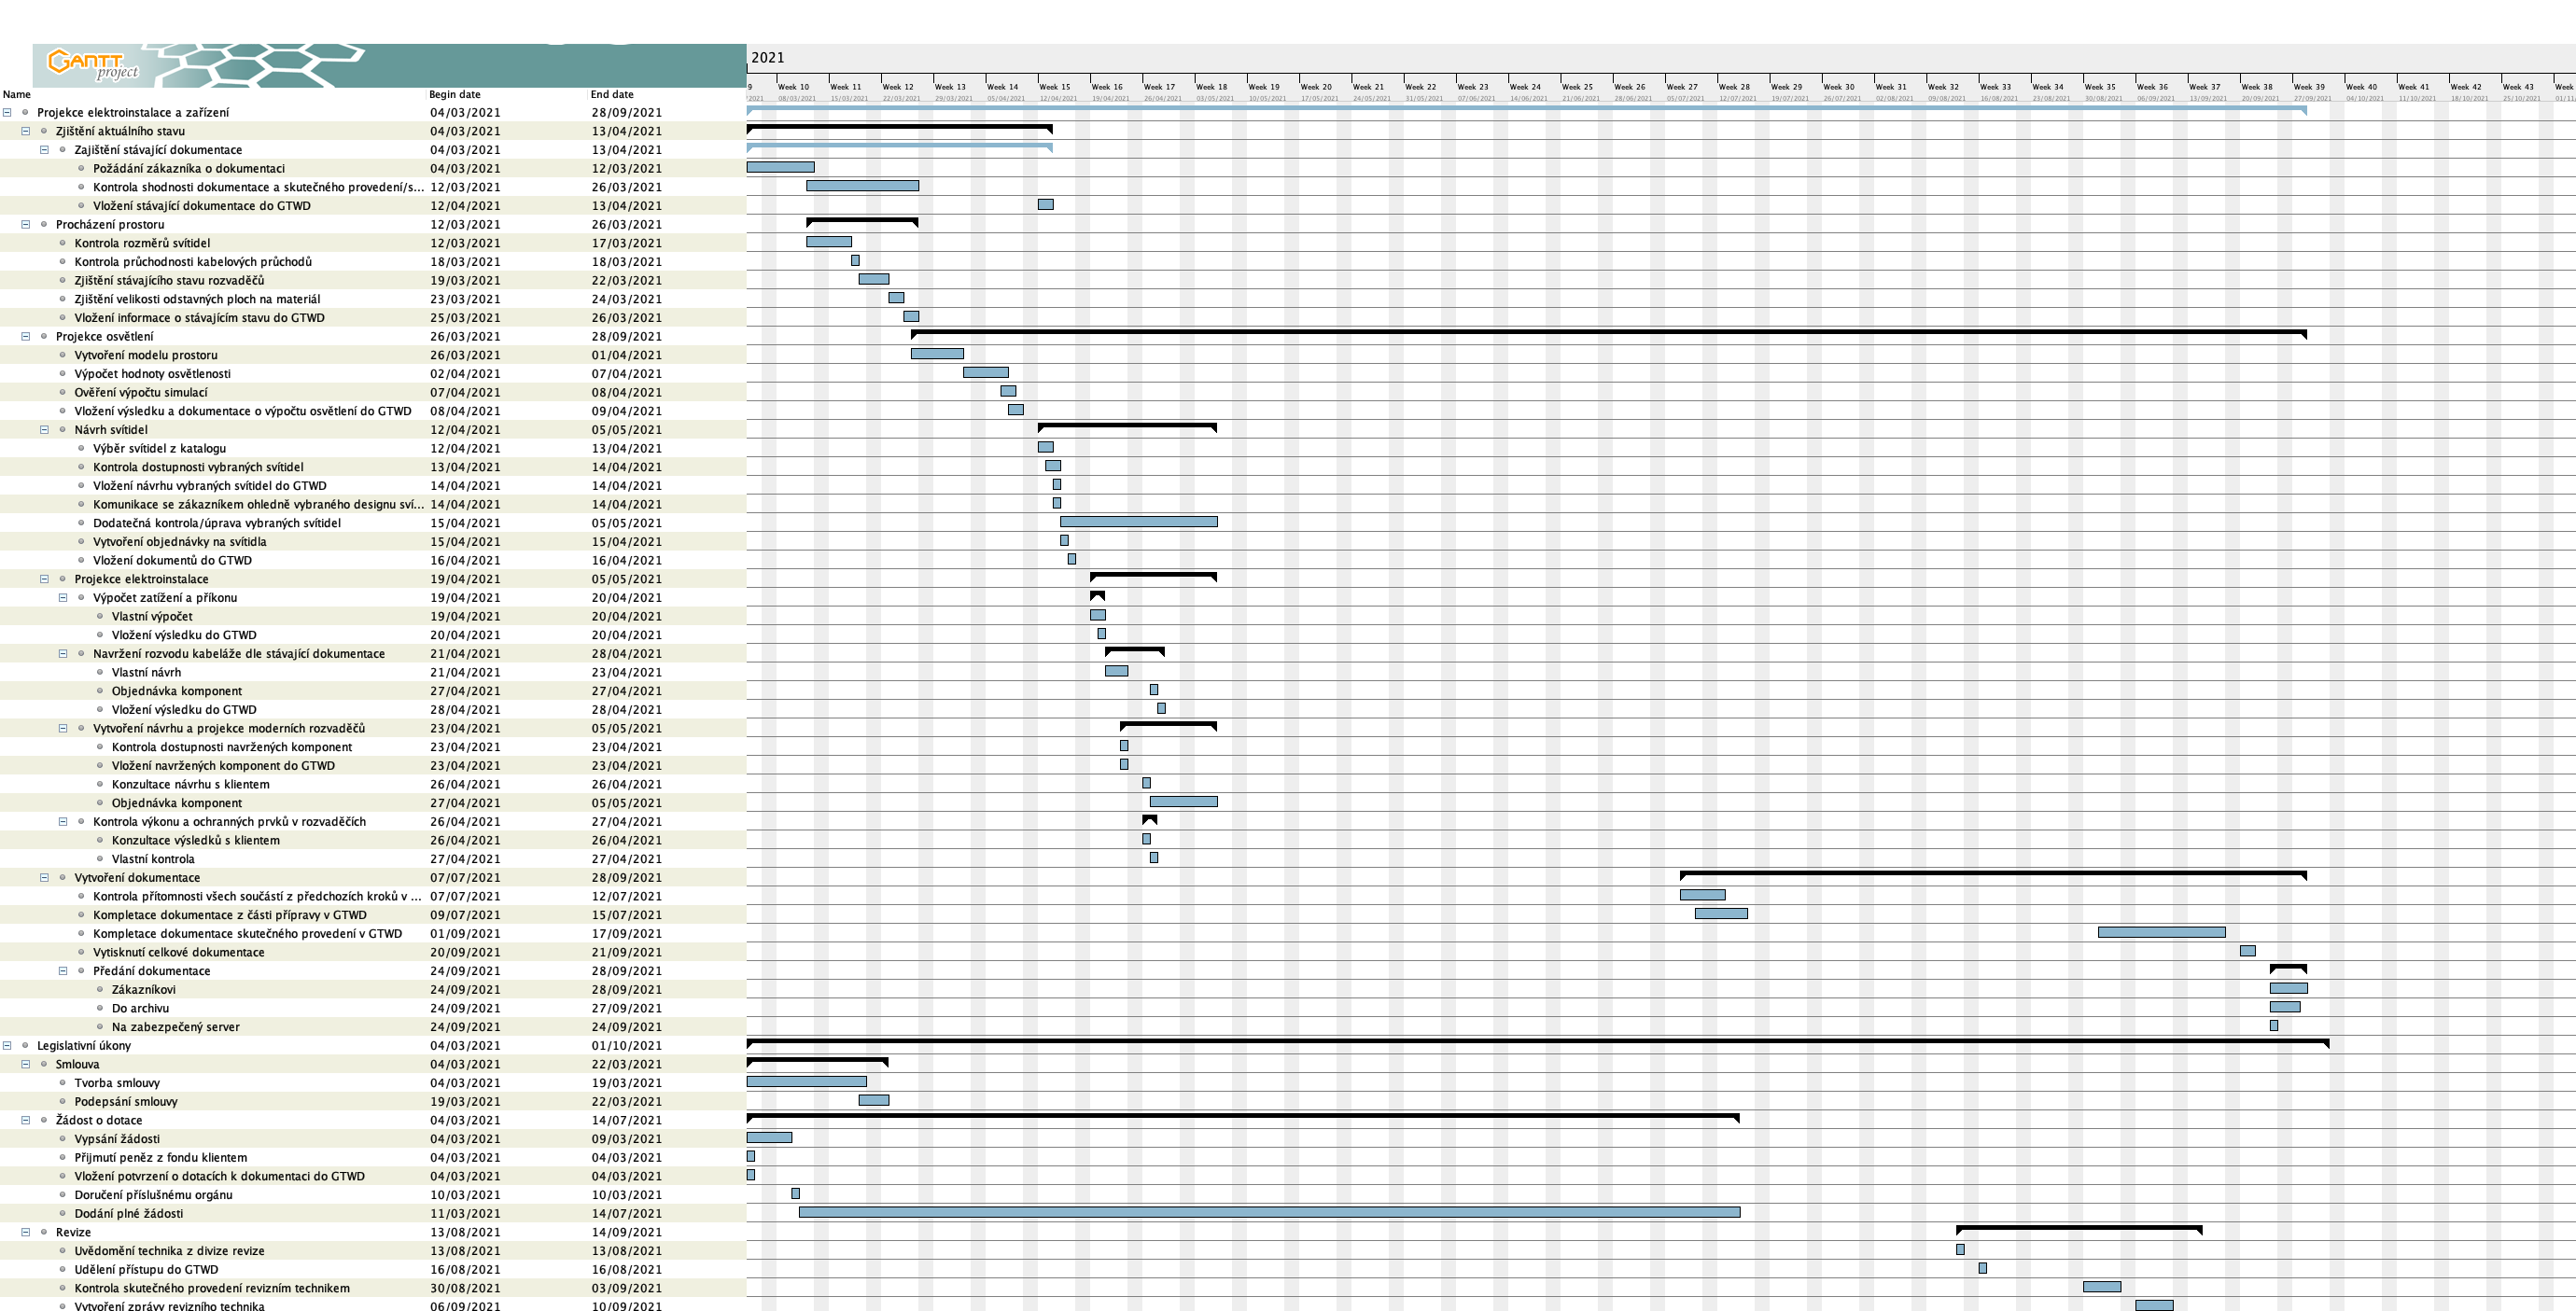
\includegraphics[width=1\textwidth]{files/gantt_half1.png} 
				\caption{GANTT 1. část}
				\label{fig:gantt_half1}
 		\end{figure}			
 		
 		\begin{figure}[H]
 				\centering
 				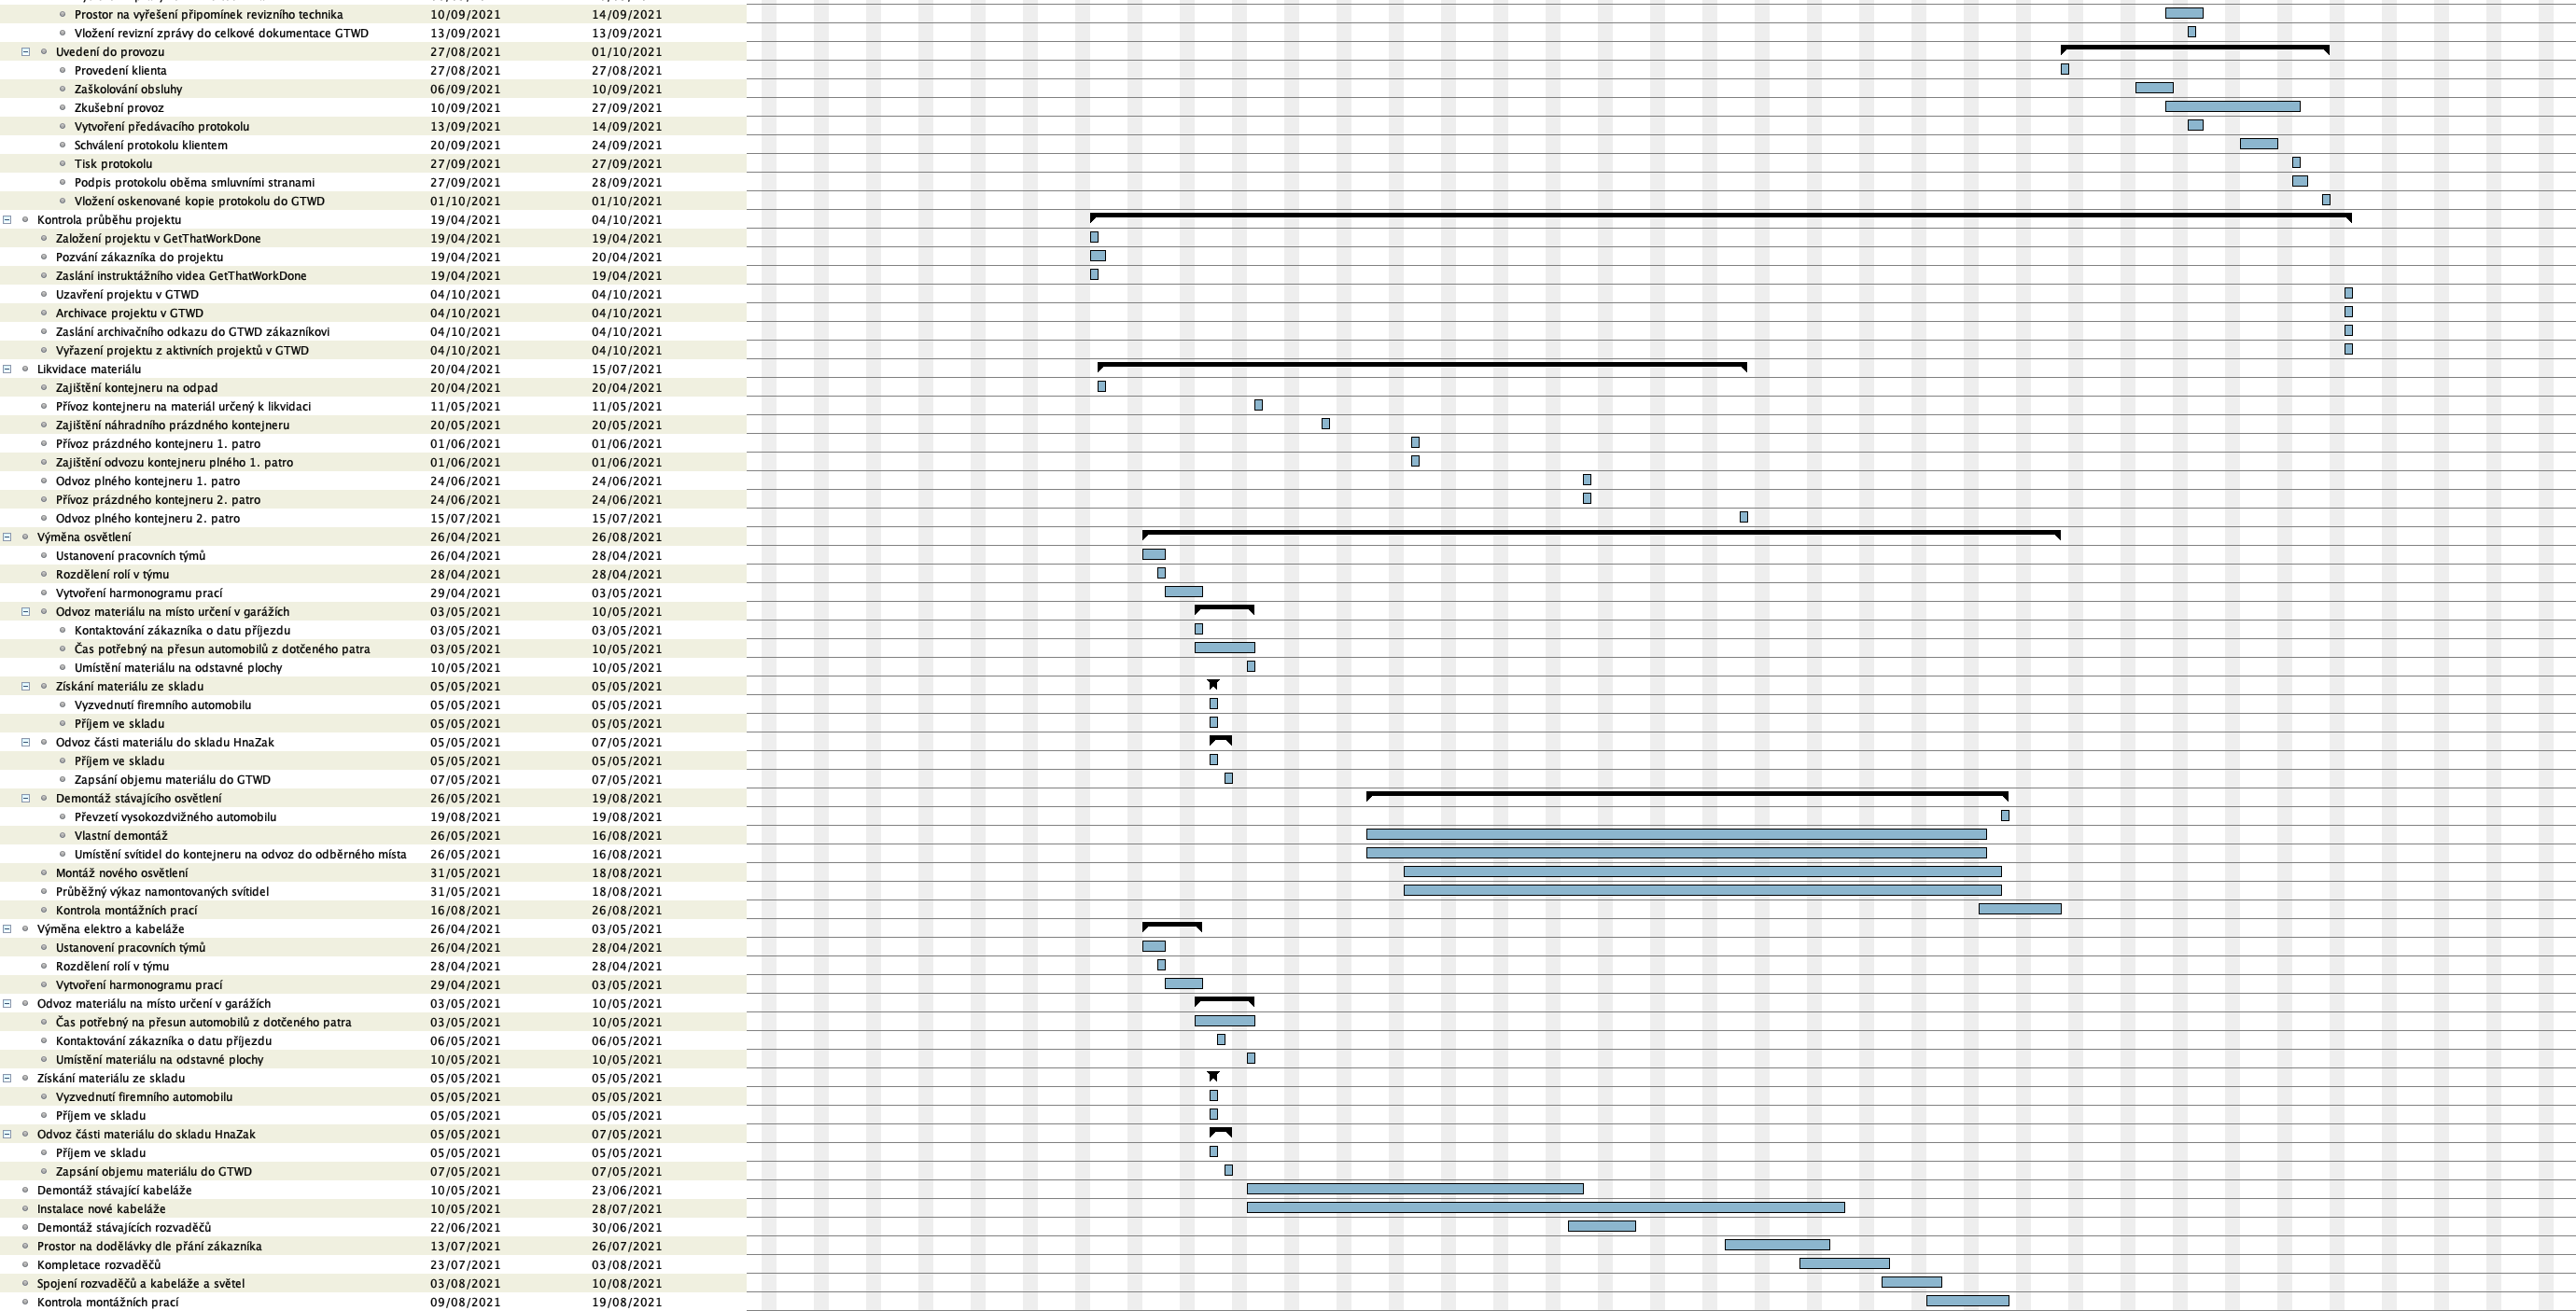
\includegraphics[width=1\textwidth]{files/gantt_half2.png} 
				\caption{GANTT 2. část}
				\label{fig:gantt_half2}
 		\end{figure}			
		
	\subsection{Analýza rizik}
	Použita metoda FMEA.
	
	\begin{table}[H]
		\resizebox{1 \textwidth}{!}
		{
		\begin{tabular}{ !{\vrule width 2pt} c !{\vrule width 2pt} p{2cm} | p{2cm} | p{2cm} | p{2cm} | c | p{2cm} | p{2cm} | p{2cm} | p{2cm} | c | p{2cm} | p{2cm} | c !{\vrule width 2pt}  }\noalign{\hrule height 2pt}
		
		\textbf{\#} & \textbf{Funkční proces} & \textbf{Potencionální poruchy (defekty)} & \textbf{Potenciální následky defektu} & \textbf{Závažnost defektu} & \textbf{Třída} & \textbf{Potenciální příčina defektu} & \textbf{Pravděpodobnost} & \textbf{Nynější řešení defektu} & \textbf{Detekovatelnost} & \textbf{RPN} & \textbf{Doporučené akce} & \textbf{Zodpovědná osoba a klíčový datum} & \textbf{Stav}   \\ \noalign{\hrule height 2pt}
	0 & žádost o~dotace & nezískání dotace & problém financování & 6 & p & nesplnění požadavků & 2 & počítáme, že dotaci získáme & 8 & 96 & získání lepších informacích o~požadavcích na dotace & právní zařizovatel & v~řešení  \  \\ \hline
	1 & dodávka materiálu & dodejka méně materiálu, než je objednáno & posunutí harmonogramu & 10 & c & nedostatek zboží u~dodavatele & 5 & posun harmonogramu & 5 & 250 & více dodavatelů s~identickým zbožím & objednavatel materiálu + externích pracích & v~řešení \  \\ \hline
	2 & dostupnost pracovníků & nedostatek pracovníků & zpoždění realizace projektu & 9 & c & neočekávaná nemoc & 3 & testování na nemoci & 5 & 135 & vakcinace & vedoucí projektu & v~plánu  \  \\ \hline
	3 & transport materiálu & materiál není přivezen na místo určení & nemožnost práce na díle & 5 & c & nedostatek automobilů & 4 & více cest pro materiál & 2 & 40 & nákup automobilů & objednavatel materiálu + externích pracích & v~plánu \  \\ \hline
	4 & dodávka materiálu & zboží není dodáno & není materiál, nemůže se projekt realizovat & 10 & c & vyčerpání zásob dodavatele & 4 & posun harmonogramu & 2 & 80 & více dodavatelů s~identickým zbožím & objednavatel materiálu + externích pracích & otázky  \  \\ \hline
	5 & dodávka svítidel & poškození svítidel & nedostatek svítidel & 5 & p & nesprávná manipulace & 3 & zakoupení více svítidel při prvotní objednávce & 1 & 15 & pevnější obaly svítidel & řídící pracovník & v~plánu  \  \\ \hline
	6 & likvidace materiálu & nemožnost likvidace & hromadění odpadu & 4 & c & přeplněné odběrné místo & 6 & transport do jiného odběrového místa & 2 & 48 & uzavření smlouvy s~odběrovým místem tak, aby vždy byla kapacita pro naše odpady & vedoucí projektu & otázky   \\ \hline
	7 & tažení kabelů & nefunkčnost kabelu & nefunkčnost instalace & 8 & p & nesprávná manipulace & 2 & výměna kabeláže & 5 & 80 & vyšší kvalifikace pracovníků & řídící pracovnk & v~řešení  \\ \hline
	8 & montáž & poničení svítidel & zvýšení finanční náročnosti & 7 & p & nesprávná manipulace & 2 &  & 3 & 42 & vyšší kvalifikace pracovníků & řídící pracovnk & v~řešení \\ \hline
	9 & revize & nesplnění požadavků & posun harmonogramu & 8 & p & nekvalitní montáž & 2 & výměna svítidla & 7 & 112 & kontrola revizním technikem již za montáže & revizní technik & v~řešení   \\ \hline
	10 & předávání instalace & zákazník odmítá dílo převzít & právní spory & 10 & n & změna managementu & 2 & neřeší se & 7 & 140 & lepší smlouva a právníci & právní zřizovatel & vyřešeno   \\ \hline
	11 & uskladnění materiálu v~OC & nemožnost uskladnění materiálu & komplikace uskladnění & 6 & n & příliš malé plochy k~uskladnění  & 5 & uskladnění ve skladě HnaZak & 3 & 90 & přesvědčení zákazníka, že další plochy je nutnost uzavřít, vyjde to levněji a ekologičtěji, než jízda pro materiál & kontaktní osoba GTWD + vedoucí projektu & v~řešení   \\ \hline
	12 & uskladnění materiálu & nemožnost uskladnění materiálu & komplikace uskladnění & 7 & c & sklad HnaZak je zaplněn & 3 & najímání skladu & 3 & 63 & rozšíření skladu & objednavatel materiálu + externích služeb & otázky   \\ \hline
	13 & komunikace se zákazníkem & zákazník nekomunikuje & nejistota zakázky & 8 & n & špatná orientace v~GTWD & 2 & telefonní kontakt & 1 & 16 & vylepšení UX GTWD & kontaktní osoba GTWD & otázky   \\ \noalign{\hrule height 2pt}
		\end{tabular}
	
		}
		\caption{FMEAT, třídy: c - řiditelné, p - procedury, n - šum}
		\end{table}
	
\section{Odbavení a podpora}
	\subsection{Plán odbavení}
	 Před podpisem proběhne maximálně třídenní školení pracovníků klienta ohledně ovládacího a monitorovacího SW osvětlení a rozvaděčů. Proběhne také potřebná instruktáž ohledně instalovaného zařízení.\par
		Zákazník, nebo jeho zástupce bude před podpisem předávacího protokolu proveden dokončeným dílem. Pokud bude mít nějaké otázky, budou mu zodpovězeny. Při průchodu bude také přítomen minimálně jeden zástupce pracovníků klienta, který absolvoval potřebné školení a instruktáž. Následně dojde k~podpisu předávacího dokumentu, předání kompletní dokumentace stávajícího stavu a všech legislativních podkladů. Žádost o~dotaci z~fondu pro revitalizaci VPO bude posouzena zpětně, vše je legislativně zařízeno, pokud dojde ke shválení žádosti, bude automaticky přispěná částka fondem připsána na zvolený účet klienta.
	\subsection{Plán podpory}
	Po jednom roce a po pěti letech od uvedení zařízení do provozu dojde k~revizi revizním technikem firmy HnaZak. Dojde také ke změření osvětlenosti, kontrole rozvaděčů, ochran a kabeláže. Pro správný chod SW na monitoring a řízení osvětlení je nutné provádět pravidelné aktualizace, proto bude zkontrolován i tento systém a popř. aktualizován na nejnovější verzi, pokud již tak nebylo provedeno zákazníkem či dříve pomocí vzdáleného ovládání.\par
	V~SW pro monitoring a řízení bude možnost přímého kontaktování podpory firmy HnaZak. Tato podpora je k~dispozici 24/7. Pokud podpora nebude schopna situaci vyřešit, dojde k~uvědomění technika ve službě. Pokud tento technik nebude schopen situaci vyřešit, budou povoláni technici, jež se na projektu podíleli.\par
	Zákazníkovi byl při předávání instalace dodán základní objem náhradních dílů a svítidel. V~případě poruchy, pokud je servisní technik OC způsobilý, je možná oprava svítidel ze strany objednatele.\par
	Pracovníci údržby zákazníka budou provádět pravidelné servisní a revizní práce. Jako základní materiál pro údržbu jim budou poskytnuty náhradní díly, která byly objednány pro montáž jako nadbytek a nebyly tudíž využity.
	\subsection{Plán odstavení}
		Odstávka instalace v~době kratší než 9 let není plánována za předpokladu, že nedojde nenadále ke změně norem, vyhlášek nebo nedojde k~zásahu vyšší moci. Po této době bude nutná opět rekonstrukce svítidel a jejich následná likvidace. Pokud nedojde k~poruše kabeláže, je možný její provoz až 20 let dle její předchozí kontroly.

	
	
\section{Vyhodnocení projektu}
	\subsection{Znovupoužitelné artefakty}
		Znovupoužitelný artefakt jsou normy, které jsme zakoupili pro studování problematiky dřívějších projektů. Využili jsme je i nyní a pokud se nezmění, využijeme je i u~příštího podobného projektu. Generalizovali jsme také UX na SW pro monitoring a řízení osvetlění a elektrické instalace. Vytvořili jsme jednotlivé moduly, které využijeme např. k~rekonstrukci rozváděčů s~podobnou technologií. Část projektové dokumentace je automatizovaná a univerzální. Pouze do ní doplňujeme potřebné informace, které je třeba zobrazit.
		%Tato dokumentace je částečně zautomatizována.
		Byla vytvořena automatická šablona na podávání žádosti o~dotace, konkrétně na příspěvek z~fondu pro revitalizaci VPO. Je však univerzální a je jí možné využít při jakékoliv standardizované žádosti o~dotace.
	\subsection{Zhodnocení tvořitelů}
	
		Tato rekonstrukce umožňuje navázání bližší spolupráce v~rámci servisu vytvářeného díla. Součástí díla nejsou servisní práce:
		
		\begin{enumerate}
			\item kontrola kabelových žlabů a stavu kabeláže, jejich vliv na přilehlé vodiče po 45 \% předpokládané doby životnosti instalace,
			\item celková kontrola svítidel po 80 \% předpokládané doby životnosti svítidel,
			\item pravidelná výměna zdrojů světla,
			\item pravidelné servisní práce rozváděčů.
		\end{enumerate}%
	\vspace*{11pt}
		Projektová dokumentace, prezentace a přílohy jsou volně dostupné v~průběhu  letního semestru 2021 na webové adrese \url{https://ptzk.cz/tpr} a slouží pouze ke studijním účelům. Jakékoliv kopírování a šíření díla bez předchozího souhlasu autorů je zakázáno. Výjimku tvoří citace.

\newpage
\printbibliography[title={{Zdroje}}]	
\nocite{*}
\addcontentsline{toc}{section}{\numberline{}Zdroje} %Added citations to TOC%

\begin{comment}
	\appendix

	\section{Příloha}
	\subsection{podkapitola přílohy}
	
\end{comment}
\end{document}
